% Format teze zasnovan je na paketu memoir
% http://tug.ctan.org/macros/latex/contrib/memoir/memman.pdf ili
% http://texdoc.net/texmf-dist/doc/latex/memoir/memman.pdf
% 
% Prilikom zadavanja klase memoir, navedenim opcijama se podešava 
% veličina slova (12pt) i jednostrano štampanje (oneside).
% Ove parametre možete menjati samo ako pravite nezvanične verzije
% mastera za privatnu upotrebu (na primer, u b5 varijanti ima smisla 
% smanjiti 
\documentclass[12pt,oneside]{memoir}

% Paket koji definiše sve specifičnosti mastera Matematičkog fakulteta
\usepackage{matfmaster}
\usepackage{amsmath}
\usepackage{amssymb}
\usepackage{arydshln}
%
% Podrazumevano pismo je ćirilica.
%   Ako koristite pdflatex, a ne xetex, sav latinički tekst na srpskom jeziku
%   treba biti okružen sa \lat{...} ili \begin{latinica}...\end{latinica}.
%
% Opicija [latinica]:
%   ako želite da pišete latiniciom, dodajte opciju "latinica" tj.
%   prethodni paket uključite pomoću: \usepackage[latinica]{matfmaster}.
%   Ako koristite pdflatex, a ne xetex, sav ćirilički tekst treba biti
%   okružen sa \cir{...} ili \begin{cirilica}...\end{cirilica}.
%
% Opcija [biblatex]:
%   ako želite da koristite reference na više jezika i umesto paketa
%   bibtex da koristite BibLaTeX/Biber, dodajte opciju "biblatex" tj.
%   prethodni paket uključite pomoću: \usepackage[biblatex]{matfmaster}
%
% Opcija [b5paper]:
%   ako želite da napravite verziju teze u manjem (b5) formatu, navedite
%   opciju "b5paper", tj. prethodni paket uključite pomoću: 
%   \usepackage[b5paper]{matfmaster}. Tada ima smisla razmisliti o promeni
%   veličine slova (izmenom opcije 12pt na 11pt u \documentclass{memoir}).
%
% Naravno, opcije je moguće kombinovati.
% Npr. \usepackage[b5paper,biblatex]{matfmaster}

% Pomoćni paket koji generiše nasumičan tekst u kojem se javljaju sva slova
% azbuke (nema potrebe koristiti ovo u pravim disertacijama)
\usepackage{pangrami}

% Paket koji obezbeđuje ispravni prikaz ćiriličkih italik slova kada
% se koristi pdflatex. Zakomentarisati ako na sistemu koji koristite ovaj
% paket nije dostupan ili ako ne radi ispravno.
\usepackage{cmsrb}

% Ostali paketi koji se koriste u dokumentu
\usepackage{listings} % listing programskog koda

% Datoteka sa literaturom u BibTex tj. BibLaTeX/Biber formatu
\bib{literatura}

% Ime kandidata na srpskom jeziku (u odabranom pismu)
\autor{Душан Пантелић}
% Naslov teze na srpskom jeziku (u odabranom pismu)
\naslov{Анализа утицаја хијерархијског усклађивања на тачност предвиђања временских серија моделима машинског учења}
% Godina u kojoj je teza predana komisiji
\godina{2026}
% Ime i afilijacija mentora (u odabranom pismu)
\mentor{др Младен \textsc{Николић}, ванредни професор\\ Универзитет у Београду, Математички факултет}
% Ime i afilijacija prvog člana komisije (u odabranom pismu)
\komisijaA{др Бојана \textsc{Милошевић}, ванредни професор\\ Универзитет у Београду, Математички факултет}
% Ime i afilijacija drugog člana komisije (u odabranom pismu)
\komisijaB{др Мирјана \textsc{Маљковић Ружичић}, доцент\\ Универзитет у Београду, Математички факултет}
% Ime i afilijacija trećeg člana komisije (opciono)
% \komisijaC{}
% Ime i afilijacija četvrtog člana komisije (opciono)
% \komisijaD{}
% Datum odbrane (obrisati ili iskomentarisati narednu liniju ako datum odbrane nije poznat)
% \datumodbrane{15. јануар 2016.}

% Apstrakt na srpskom jeziku (u odabranom pismu)
\apstr{%
Управљање ланцима снабдевања захтева прецизно предвиђање потражње на више нивоа агрегације, што је значајно отежано изразитом испрекиданошћу временских серија. Циљ овог рада био је да се испита утицај различитих метода хијерархијског усклађивања на прецизност базних прогноза и квантификује губитак математичке кохерентности приликом хеуристичког третмана негативних вредности. Истраживање је спроведено на скупу од 20.000 временских серија, уз евалуацију једанаест алгоритама (од статистичких модела до савремених вишенаменских претренираних мрежа). Базне прогнозе су подвргнуте структурном и темпоралном усклађивању (\textit{OLS}, \textit{WLS\_Struct}, \textit{WLS\_Var}, \textit{MinT\_Shrink}), уз упоредну анализу строге оптимизације (QP) и хеуристичког одсецања негативних вредности на нулу. Резултати показују да усклађивање не побољшава универзално тачност система. Вишенаменски претренирани модели (\textit{Chronos}, \textit{TimesFM}) остварују најбоље перформансе, док детерминистичко усклађивање (\textit{OLS}) драстично деградира њихов прецизан локални сигнал. Показано је да темпорално усклађивање функционише примарно као пост-хок регуларизатор који значајно ублажава грешке изразито лоших модела (пад грешке до $60\%$ код \textit{LightGBM}-а), али истовремено квари сигнале прецизних алгоритама. Такође, доказано је да хеуристичко одсецање негативних прогноза доводи до просечног нарушавања кохерентности од $6.00\%$, што се применом методе \textit{WLS\_Var} своди на занемарљивих $0.5\%$. Закључак указује да хеуристичко одсецање негативних вредности, упарено са методама које поштују историјску варијансу, представља бољу праксу од нестабилних QP решавача, пружајући директне смернице за пројектовање робусних предиктивних система у разматраном домену.
}

% Ključne reči na srpskom jeziku (u odabranom pismu)
\kljucnereci{хијерархијске временске серије, хијерархијско усклађивање, предвиђање временских серија, испрекидана потражња, машинско учење, дубоко учење, вишенаменски претренирани модели, статистички модели}

\begin{document}
% ==============================================================================
% Uvodni deo teze
\frontmatter
% ==============================================================================
% Naslovna strana
\naslovna
% Strana sa podacima o mentoru i članovima komisije
\komisija
% Strana sa posvetom (u odabranom pismu)
% \posveta{Мами, тати и деди}
% Strana sa podacima o disertaciji na srpskom jeziku
\apstrakt
% Sadržaj teze
\tableofcontents*

% ==============================================================================
% Glavni deo teze
\mainmatter
% ==============================================================================

% ------------------------------------------------------------------------------
\chapter{Увод}
% ------------------------------------------------------------------------------

Предвиђање (прогнозирање) временских серија (енг. time series forecasting) представља фундаменталну област машинског учења и примењене статистике, која за циљ има екстракцију образаца из секвенцијалних података. Иако ови концепти налазе примену у разним доменима, од обраде сигнала до метеорологије, њихов највећи практични утицај је у домену пословних система и ланаца снабдевања \cite{makridakis2020m4}. Данашње свакодневно пословно окружење карактерише изузетна динамичност, која је резултат непредвидивости и све веће сложености тржишта. Способност организација да доносе правовремене одлуке на основу предвиђања будућих догађаја директно утиче на њихову стабилност и конкурентност. Међутим, реални подаци који описују пословне системе ретко су изоловане временске серије. Наиме, подаци унутар једне организације готово увек поседују инхерентну хијерархијску или групну структуру. Усклађивање ових процеса кроз све нивое одлучивања представља један од највећих изазова \cite{hyndman2021forecasting}.

\section{Контекст и значај проблема и области}

Предвиђање у системима са хијерархијама захтева предвиђање догађаја на различитим нивоима агрегације.  Хијерархије се могу поделити на  две основне димензије:

\begin{enumerate}
\item \textbf{Структуралне:} Представљају просторну или логичку агрегацију, односно декомпозицију података у фиксном временском интервалу. На пример, у глобалном ланцу снабдевања, укупна светска тражња се декомпонује на регионе, државе, дистрибутивне центре, и на крају на појединачне артикле (енг. stock keeping unit – SKU).
\item \textbf{Временске:} Подразумевају агрегацију података високе учесталости (нпр. дневне трансакције) у ниже фреквенције (недељне, месечне, годишње серије), што омогућава моделовањe краткорочних оперативних осцилација и дугорочних стратешких трендова \cite{athanasopoulos2017forecasting}.
\end{enumerate}

Традиционално се овом проблему приступа применом хеуристичких метода. Приступ "од дна ка врху" (енг. bottom-up) предвиђа само најниже нивое који се потом сабирају, али је изузетно осетљив на висок ниво шума карактеристичан за податке на ниском нивоу  \cite{dangerfield1992bottom}. Са друге стране, приступ "од врха ка дну" (енг. top-down) користи стабилност агрегираних података на вишим нивоима \cite{gross1990disaggregation}, али често не успева да прецизно декомпонује информације, губећи битне локалне карактеристике података \cite{athanasopoulos2009hierarchical}. Независно генерисане прогнозе на различитим нивоима су по правилу математички некохерентне (збир нижих нивоа не одговара прогнози вишег нивоа), што може довести до контрадикторних пословних одлука.

Као примарно решење овог проблема развијена је парадигма оптималног усклађивања (енг. optimal reconciliation) \cite{hyndman2011optimal}, са методом минималног трага (енг. minimum trace – MinT) као тренутним стандардом \cite{wickramasuriya2019optimal}. Иако је иницијални мотив за развој ових метода била административна кохерентност, новија сазнања указују на то да усклађивање заправо функционише као механизам регуларизације \cite{kourentzes2019cross}. Приморавањем модела са различитих нивоа да "комуницирају", усклађивање омогућава пренос информација, стабилност и ниска варијанса са виших нивоа хијерархије спуштају се на нижи ниво, док се карактеристични сигнали са дна пењу ка врху. Управо ова информациона размена, а не пука математичка кохерентност, представља потенцијал за унапређење предиктивних система.

Досадашња литература је овај домен претежно анализирала кроз употребу класичних модела машинског учења и статистичких модела. Скорашњи напредак архитектура дубоког учења \cite{lim2021temporal, oreshkin2019nbeats}, као и појава тзв. вишенаменских претренираних (енг. foundation) модела обучених на великим скуповима података \cite{ansari2024chronos, das2023timesfm}, захтевају потпуно нову евалуацију у контексту хијерархијског усклађивања.

\section{Дефиниција истраживачког проблема}

Суштина истраживачког проблема лежи у промени парадигме: усклађивање независних прогноза се у овом раду не посматра искључиво као захтев за изједначавање збирова, већ као механизам за побољшање предвиђања кроз размену информација између нивоа хијерархије. Проблем се огледа у проналажењу оптималног математичког модела који ће ово омогућити. Метод минималног трага постиже размену информација ослањајући се на апроксимацију матрице коваријансе грешака ван узорка, помоћу података из узорка (резидуала или историјских вредности). Међутим, примена ове методологије на реалне податке открива неколико изазова којима се овај рад првенствено бави:

\begin{enumerate}
\item \textbf{Проблем апроксимације структуре грешака:} Иако увођење пуне узорачке матрице коваријансе (основна варијанта методе минималног трага) теоријски омогућава најпотпунији пренос информација, њена примена на хијерархије са великим бројем временских серија је статистички и нумерички нестабилна. Када број временских серија (20.000) драстично превазилази број расположивих историјских опажања ($\sim$60), пуна узорачка матрица коваријансе постаје непотпуног ранга и сингуларна, што онемогућава њену инверзију \cite{schafer2005shrinkage}. Услед ових ограничења, варијанте са пуном узорачком коваријансом су искључене из анализе. Истраживање се фокусира на евалуацију преосталих стабилних алтернатива: OLS (метод обичних најмањих квадрата) и WLS\_Struct (метод пондерисаних најмањих квадрата заснован на структури хијерархије) које нестабилност заобилазе ослањајући се на геометрију и топологију хијерархије без анализе грешака, WLS\_Var (метод пондерисаних најмањих квадрата заснован на варијанси) која уводи само дијагоналне варијансе резидуала,  као и напредне регуларизационе технике MinT\_Shrink, која поступком математичког „скупљања” (енг. shrinkage) стабилизује пуну матрицу коваријансе.

\item \textbf{Сукоб математичке кохерентности и физичких ограничења:} Усклађивање често резултује негативним прогнозама, што је у контексту прогнозирања потражње физички немогуће и доводи до деградације евалуационих метрика. Формална ограничења ненегативности се успешно имплементирају кроз квадратно програмирање, односно оптимизацију, што за последицу има прелазак са аналитичког решења на итеративно тражење оптимума. Овај прелазак уводи озбиљне нумеричке изазове и рачунарску комплексност у условима високе димензионалности и ограниченог историјског узорка. Иако ова појава зависи од специфичне топологије података и резидуала, она у оквиру нашег експеримента узрокује да итеративни поступци за емпиријске методе (WLS\_Var и MinT\_Shrink) доживљавају нумеричку нестабилност услед лоше условљености матрица израчунатих из резидуала.  Насупрот њима, детерминистичке методе (OLS и WLS\_Struct) успешно конвергирају на нашим подацима. С обзиром на то да овај рад евалуира перформансе модела и са формалним ограничењима и кроз стратегију хеуристичког одсецања негативних вредности на нулу (енг. clipping to zero), отвара се истраживачко питање: Како избор између строге математичке кохерентности и накнадних интервенција утиче на прецизност прогноза на циљаном (базном) нивоу и да ли се задржавају бенефити преноса информација?

\item \textbf{Хетерогеност структура грешака:} Различите класе модела генеришу суштински различите обрасце резидуала. Истраживачки изазов је разумевање интеракције ове хетерогености унутар метода за усклађивање и како утичу на коначан резултат.
\end{enumerate}


\section{Примарни циљеви рада}

Да би се успешно одговорило на дефинисани истраживачки проблем, постављени су следећи примарни циљеви:

\begin{enumerate}
 \item \textbf{Системска евалуација примењивих варијанти MinT:} Спровести свеобухватну компаративну анализу четири методе усклађивања (\textit{OLS}, \textit{WLS\_Struct}, \textit{WLS\_Var} и \textit{MinT\_Shrink}) на структуралним и временским хијерархијама.
    
  \item \textbf{Анализа утицаја ограничења ненегативности:} Испитати како увођење формалних ограничења ненегативности (за \textit{OLS} и \textit{WLS\_Struct}), у поређењу са стратегијом накнадног хеуристичког одсецања негативних вредности на нулу утиче на метрике. Циљ је демонстрирати да се предности размене информација кроз нивое могу задржати чак и када је строга математичка кохерентност делимично нарушена ради очувања пословне логике и рачунарских перформанси.
    
\item \textbf{Компаративна евалуација четири фамилије предиктивних модела:} 
    \begin{itemize}
        \item Статистички модели (\textit{ARIMA}, \textit{Holt-Winters}, \textit{Prophet}).
        \item Класични модели машинског учења (\textit{LightGBM}, \textit{RandomForest}).
        \item Модели дубоког учења (\textit{DeepAR}, \textit{N-HITS}).
        \item Вишенаменски претренирани модели за временске серије (\textit{Chronos}, \textit{TimesFM}).
    \end{itemize}
    
 \item \textbf{Идентификација најбољих пракси:} Синтетизовати резултате у јасне смернице које ће допринети лакшем избору оптималне комбинације модела, методе усклађивања и стратегије третмана негативних прогноза у реалним пословним системима.
\end{enumerate}

\section{Кључни резултати}

Темељна експериментална евалуација спроведена у овом раду довела је до неколико увида:

\begin{itemize}
    \item \textbf{Супериорност савремених архитектура:} На посматраном скупу података, вишенаменски претренирани модели и вероватносне неуронске мреже вишеструко надмашују класичне алгоритме машинског учења. Стабла одлучивања са стандардном функцијом циља показују велику пристрасност и нису адекватна за серије са великим бројем нула.
    
    \item \textbf{Ограничења хијерархијског усклађивања:} Показано је да усклађивање не побољшава аутоматски прецизност базних прогноза. Детерминистички приступи најчешће деградирају прецизне локалне сигнале, док је квалитет добрих модела могуће сачувати искључиво применом метода које интелигентно скалирају корекције.
    
    \item \textbf{Темпорално усклађивање као регуларизатор:} Усклађивање кроз време не доноси стварну предиктивну вредност већ оптималним алгоритмима. Оно делује примарно као механизам пост-хок регуларизације који ублажава екстремне грешке модела лошијих перформанси.
    
    \item \textbf{Оправданост инжењерског компромиса:} Показано је да строга математичка оптимизација за спречавање негативних прогноза није рачунарски одржива у високодимензионалним корпоративним системима. Једноставно хеуристичко одсецање негативних вредности представља бољи правац, јер обезбеђује физички смислене прогнозе уз занемарљив губитак агрегационе кохерентности.
    
    \item \textbf{Утицај дизајна хијерархије:} Комплекснија структура хијерархије уноси додатни шум у систем. Редуковање броја агрегационих нивоа значајно ублажава деградацију базних прогноза услед смањеног броја алгебарских ограничења.
\end{itemize}

Остатак рада је структуриран у четири поглавља. У поглављу 2 изложене су теоријске основе хијерархијских временских серија и методе за њихово усклађивање. Поглавље 3 описује експерименталну поставку, коришћени скуп података, архитектуре модела и метрике евалуације. У поглављу 4 приказани су резултати експеримената уз пратећу дискусију, док су у поглављу 5 изведени главни закључци и дате смернице за даља истраживања.

% ------------------------------------------------------------------------------
\chapter{Теоријске основе}
\label{chp:teorijske_osnove}
% ------------------------------------------------------------------------------

Ово поглавље поставља формални математички и статистички оквир неопходан за разумевање проблема предвиђања у сложеним системима. Први део поглавља уводи основне концепте временских серија. Затим се дефинишу алгебарске структуре хијерархијских и груписаних временских серија. Коначно, трећи део поглавља доноси детаљан теоријски преглед метода за усклађивање предвиђања.

\section{Основни концепти предвиђања временских серија}

Временска серија се математички дефинише као низ опажања посматраних у узастопним, најчешће једнако удаљеним временским интервалима. Нека је $y_t$ вредност посматране променљиве у тренутку $t$. Временска серија дужине $T$ може се представити као секвенца $\mathbf{y} = (y_1, y_2, \dots, y_T)$. Циљ предвиђања (прогнозирања) јесте процена будућих вредности, које означавамо са $\hat{y}_{T+h}$ за $h = 1, 2, \dots, H$, где $h$ представља хоризонт предвиђања, на основу историјских података и потенцијалних екстерних фактора \cite{hyndman2021forecasting}.

Иако класична теорија временских серија често посматра податке кроз експлицитне декомпозиције на тренд, сезоналност и шум, у савременим предиктивним системима, моделима се најчешће прослеђује сирова, недекомпонована серија. Без обзира на то да ли припадају фамилији статистичких метода, алгоритмима машинског учења, или архитектурама дубоког учења, од модела се очекује да самостално екстрахују релевантне темпоралне информације директно из оригиналног сигнала.

У контексту ланаца снабдевања, посебан изазов представљају подаци на најнижим нивоима агрегације који некада попримају облик \textbf{испрекиданих временских серија}. Испрекидане серије карактерише велики број нултих вредности (периоди без икакве потражње) испрекидан повременим, често варијабилним позитивним вредностима када се потражња заправо деси. 

Управо ово својство чини предвиђање серија изузетно тешким и подложним високом нивоу шума, што потенцијално можемо решити  позајмљивањем стабилнијих информација са виших нивоа агрегације кроз процес хијерархијског усклађивања (где се скуп индивидуалних серија $y_t$ третира као јединствен систем више променљивих $\mathbf{y}_t$), како би се побољшале предикције на целом систему.

\section{Хијерархијске и груписане временске серије}

У реалним пословним системима, временске серије нису изоловани ентитети, већ су међусобно повезане строгим правилима агрегације. Ове структуре се генерално деле на хијерархијске (где постоји строги редослед рашчлањивања, нпр. држава $\rightarrow$ регион $\rightarrow$ град) и груписане (где се подаци могу агрегирати по више независних атрибута, нпр. агрегација по географској локацији или алтернативно по типу производа).

\subsection{Математичка формулација структуралних хијерархија}

Нека систем садржи укупно $n$ временских серија, од којих се $m$ серија налази на најнижем (базном) нивоу, док преосталих $k = n - m$ серија представљају агрегиране вредности на вишим нивоима. 

Вектор свих опажања у тренутку $t$, означен са $\mathbf{y}_t$ (димензија $n \times 1$), може се партиционисати на вектор агрегираних серија $\mathbf{a}_t$ (димензија $k \times 1$) и вектор базних серија $\mathbf{b}_t$ (димензија $m \times 1$):
\begin{equation}
    \mathbf{y}_t = \begin{bmatrix} \mathbf{a}_t \\ \mathbf{b}_t \end{bmatrix}
\end{equation}

Кључни алгебарски елемент који дефинише структуру овог система јесте \textbf{матрица сабирања $\mathbf{S}$} (енг. \textit{summing matrix}) димензија $n \times m$. Ова матрица пресликава базне серије у све остале серије у систему. Коришћењем матрице $\mathbf{S}$, цео систем се може изразити искључиво преко базних серија:
\begin{equation}
    \mathbf{y}_t = \mathbf{S} \mathbf{b}_t
\end{equation}

Матрица $\mathbf{S}$ се може партиционисати као:
\begin{equation}
    \mathbf{S} = \begin{bmatrix} \mathbf{A} \\ \mathbf{I}_m \end{bmatrix}
\end{equation}
где је $\mathbf{A}$ агрегациона матрица димензија $k \times m$ која дефинише како се базне серије сабирају да би се добили виши нивои, док је $\mathbf{I}_m$ јединична матрица димензија $m \times m$ која пресликава базне серије саме на себе. Елементи матрице $\mathbf{A}$ су типично бинарни (0 или 1), где 1 означава да базна серија припада одговарајућем сумирању.

Да би се илустровала моћ и флексибилност ове формулације, у наставку су приказана два карактеристична примера: један за стриктну хијерархију и један за груписане серије.

\vspace{1em}
\noindent \textbf{Пример 1: Стриктна хијерархија (стабло)} \\
Посматрајмо систем са три нивоа, где је укупна продаја државе (највиши ниво, $y_T$) декомпонована на два региона: север ($y_S$) и југ ($y_J$). Даље, регион север чине два града ($y_{S1}, y_{S2}$), а регион југ такође два града ($y_{J1}, y_{J2}$). Ово је класична структура стабла где су нижи нивои стриктни подскупови виших.

У овом систему имамо $m=4$ базне серије (градови) и укупно $n=7$ серија. Матрица сабирања $\mathbf{S}$ димензија $7 \times 4$ формира се на следећи начин:
\begin{equation}
    \begin{bmatrix} 
    y_T \\ \hline
    y_S \\ 
    y_J \\ \hline
    y_{S1} \\
    y_{S2} \\
    y_{J1} \\
    y_{J2}
    \end{bmatrix} 
    = 
    \underbrace{
    \begin{bmatrix} 
    1 & 1 & 1 & 1 \\ \hline
    1 & 1 & 0 & 0 \\ 
    0 & 0 & 1 & 1 \\ \hline
    1 & 0 & 0 & 0 \\
    0 & 1 & 0 & 0 \\
    0 & 0 & 1 & 0 \\
    0 & 0 & 0 & 1 
    \end{bmatrix}
    }_{\mathbf{S}}
    \begin{bmatrix} 
    y_{S1} \\ 
    y_{S2} \\
    y_{J1} \\
    y_{J2}
    \end{bmatrix}
\end{equation}
Горња три реда представљају агрегациону матрицу $\mathbf{A}$, док су доња четири реда јединична матрица $\mathbf{I}_4$.

\vspace{1em}
\noindent \textbf{Пример 2: Груписане временске серије} \\
За разлику од стриктне хијерархије, подаци се често могу груписати по више независних атрибута. Претпоставимо да компанија прати продају по географском региону (регион А и регион Б) и алтернативно по категорији производа (производ X и производ Y). 

Најнижи (базни) ниво чине све комбинације ових атрибута ($y_{AX}, y_{AY}, y_{BX}, y_{BY}$), што даје $m=4$. Виши нивои чине: укупна продаја ($y_T$), укупна продаја по регионима ($y_A, y_B$) и укупна продаја по производима ($y_X, y_Y$). Укупно имамо $n=9$ серија. Mатрица сабирања $\mathbf{S}$ сада изгледа овако:
\begin{equation}
    \begin{bmatrix} 
    y_T \\ \hline
    y_A \\ 
    y_B \\ \hline
    y_X \\
    y_Y \\ \hline
    y_{AX} \\
    y_{AY} \\
    y_{BX} \\
    y_{BY}
    \end{bmatrix} 
    = 
    \underbrace{
    \begin{bmatrix} 
    1 & 1 & 1 & 1 \\ \hline
    1 & 1 & 0 & 0 \\ 
    0 & 0 & 1 & 1 \\ \hline
    1 & 0 & 1 & 0 \\
    0 & 1 & 0 & 1 \\ \hline
    1 & 0 & 0 & 0 \\
    0 & 1 & 0 & 0 \\
    0 & 0 & 1 & 0 \\
    0 & 0 & 0 & 1 
    \end{bmatrix}
    }_{\mathbf{S}}
    \begin{bmatrix} 
    y_{AX} \\ 
    y_{AY} \\
    y_{BX} \\
    y_{BY}
    \end{bmatrix}
\end{equation}
Док редови за регионе врше класично сабирање суседних елемената (као у примеру 1), редови за производе ($y_X$ и $y_Y$) врше унакрсно сабирање (нпр. $y_X = y_{AX} + y_{BX}$). Целокупна комплексност било стриктне хијерархије, било унакрсног груписања, садржана је унутар структуре матрице $\mathbf{S}$.

\subsection{Временске хијерархије}

Поред структуралне агрегације, временске серије се могу посматрати кроз призму временских хијерархија \cite{athanasopoulos2017forecasting}. Ако претпоставимо да располажемо подацима високе фреквенције, ова опажања се могу агрегирати у ниже фреквенције. Временска хијерархија омогућава да се шум у високофреквентним подацима ублажи кроз агрегацију, док нискофреквентни подаци олакшавају моделирање дугорочних трендова. 

Концепт изоморфизма између структуралних и временских хијерархија може се приказати на примеру агрегације високофреквентних \textbf{месечних података у нискофреквентну кварталну серију} (што уједно одговара и временској агрегацији примењеној у овом истраживању).

Нека су $y_{M1}, y_{M2}, y_{M3}$ опажања за три узастопна месеца (базне серије у временском домену), а $y_{Q1}$ њихова укупна квартална вредност (агрегирана серија). Временски вектор система за овај квартал је $\mathbf{y}_{temp} = \begin{bmatrix} y_{Q1} & y_{M1} & y_{M2} & y_{M3} \end{bmatrix}^T$. 

Припадајућа матрица сабирања $\mathbf{S}_{temp}$ димензија $4 \times 3$ формира се по идентичном принципу:
\begin{equation}
    \begin{bmatrix} 
    y_{Q1} \\ \hline
    y_{M1} \\ 
    y_{M2} \\
    y_{M3} 
    \end{bmatrix} 
    = 
    \begin{bmatrix} 
    1 & 1 & 1 \\ \hline
    1 & 0 & 0 \\ 
    0 & 1 & 0 \\
    0 & 0 & 1 
    \end{bmatrix}
    \begin{bmatrix} 
    y_{M1} \\ 
    y_{M2} \\
    y_{M3} 
    \end{bmatrix}
\end{equation}

Кроз ове примере јасно се уочава да без обзира на то да ли се подаци агрегирају просторно или темпорално, алгебарска структура проблема (релација $\mathbf{y} = \mathbf{S}\mathbf{b}$) остаје потпуно иста. Ово својство омогућава примену идентичних алгоритама за оптимално усклађивање како на просторној, тако и на временској димензији.


\section{Методе за усклађивање предвиђања}

Када се за сваку серију у хијерархији независно генерише предвиђање, добијамо вектор неусклађених прогноза $\hat{\mathbf{y}}_t$. Због независне природе предиктивних процеса, ове прогнозе готово никада не задовољавају хијерархијску структуру, односно:
\begin{equation}
    \hat{\mathbf{y}}_t \neq \mathbf{S}\tilde{\mathbf{b}}_t
\end{equation}
Овај недостатак кохерентности решава се приступом усклађивања.

\subsection{Општи оквир усклађивања и традиционалне методе}

Све линеарне методе усклађивања могу се представити као линеарне трансформације које пресликавају независне прогнозе у нове вредности које строго задовољавају правила хијерархијске агрегације.
Комплетан вектор усклађених прогноза $\tilde{\mathbf{y}}_t$, који садржи ревидиране вредности за све серије на свим нивоима система, добија се применом следеће линеарне трансформације на вектор неусклађених прогноза $\hat{\mathbf{y}}_t$:
\begin{equation}
    \tilde{\mathbf{y}}_t = \mathbf{S} \mathbf{P} \hat{\mathbf{y}}_t
\end{equation}
Математички посматрано, ова трансформација се одвија у два логичка корака. Прво, пројекциона матрица $\mathbf{P}$ (димензија $m \times n$) узима информације из неусклађених прогноза са свих нивоа ($\hat{\mathbf{y}}_t$) и пресликава их у вектор кохерентних прогноза на основном (базном) нивоу. Затим, множењем са матрицом сабирања $\mathbf{S}$, те усклађене базне прогнозе се агрегирају. Коначни резултат ове операције ($\tilde{\mathbf{y}}_t$) јесте потпуно усклађен систем у коме су прогнозе на свим нивоима хијерархије математички конзистентне. Иако је у пракси базни ниво најчешће примарни циљ за евалуацију предиктивних метрика и оперативну реализацију, процес усклађивања унапређује и синхронизује цео систем.

Овај алгебарски оквир је универзалан \cite{wickramasuriya2019optimal}. Све традиционалне, хеуристичке методе усклађивања могу се представити специфичним избором елемената унутар матрице $\mathbf{P}$:

\vspace{1em}
\noindent \textbf{Приступ од дна ка врху:} \\
Ова метода, која представља један од најстаријих приступа у хијерархијском прогнозирању, претпоставља да су прогнозе на најнижем нивоу једине релевантне, док се прогнозе генерисане на вишим нивоима потпуно игноришу \cite{dangerfield1992bottom}. Усклађене прогнозе виших нивоа добијају се искључиво сабирањем базних прогноза. Матрица $\mathbf{P}$ за ову методу дефинише се као:
\begin{equation}
    \mathbf{P}_{BU} = \begin{bmatrix} \mathbf{0}_{m \times k} & \mathbf{I}_m \end{bmatrix}
\end{equation}
где је $\mathbf{0}_{m \times k}$ нулти блок који множи и поништава све прогнозе са виших нивоа (укупно $k$ серија), док јединична матрица $\mathbf{I}_m$ пропушта базне прогнозе непромењене. 

Да бисмо ово илустровали на примеру 1 из претходног поглавља (где имамо $n=7$ серија и $m=4$ града као базне серије), вектор свих неусклађених прогноза је $\hat{\mathbf{y}}_t = [\hat{y}_T, \hat{y}_S, \hat{y}_J, \hat{y}_{S1}, \hat{y}_{S2}, \hat{y}_{J1}, \hat{y}_{J2}]^T$. Матрица $\mathbf{P}_{BU}$ димензија $4 \times 7$ изгледа овако:
\begin{equation}
    \mathbf{P}_{BU} = 
    \begin{bmatrix}
    0 & 0 & 0 & \vline & 1 & 0 & 0 & 0 \\
    0 & 0 & 0 & \vline & 0 & 1 & 0 & 0 \\
    0 & 0 & 0 & \vline & 0 & 0 & 1 & 0 \\
    0 & 0 & 0 & \vline & 0 & 0 & 0 & 1
    \end{bmatrix}
\end{equation}
Множењем $\mathbf{P}_{BU} \hat{\mathbf{y}}_t$, прве три колоне (нулти блок) потпуно елиминишу прогнозе $\hat{y}_T, \hat{y}_S, \hat{y}_J$, остављајући само четири базне прогнозе које се затим преко матрице $\mathbf{S}$ сабирају навише. Главни недостатак овог приступа је очигледан: огромна количина информација са врха хијерархије се просто одбацује.

\vspace{1em}
\noindent \textbf{Приступ од врха ка дну:} \\
Ова метода ради потпуно супротно: узима у обзир искључиво прогнозу са највишег (глобалног) нивоа, док игнорише све остале \cite{gross1990disaggregation}. Глобална прогноза се затим дистрибуира на ниже нивое помоћу вектора историјских пропорција $\mathbf{p} = [p_1, p_2, \dots, p_m]^T$, где важи $\sum_{i=1}^{m} p_i = 1$. Матрица $\mathbf{P}$ за ову методу има облик:
\begin{equation}
    \mathbf{P}_{TD} = \begin{bmatrix} \mathbf{p} & \mathbf{0}_{m \times (n-1)} \end{bmatrix}
\end{equation}
Ако ово применимо на исти пример 1 са 7 серија, и претпоставимо да смо израчунали вектор пропорција $\mathbf{p} = [p_{S1}, p_{S2}, p_{J1}, p_{J2}]^T$ (нпр. на основу просечне историјске продаје сваког града), матрица $\mathbf{P}_{TD}$ изгледа овако:
\begin{equation}
    \mathbf{P}_{TD} = 
    \begin{bmatrix}
    p_{S1} & \vline & 0 & 0 & 0 & 0 & 0 & 0 \\
    p_{S2} & \vline & 0 & 0 & 0 & 0 & 0 & 0 \\
    p_{J1} & \vline & 0 & 0 & 0 & 0 & 0 & 0 \\
    p_{J2} & \vline & 0 & 0 & 0 & 0 & 0 & 0
    \end{bmatrix}
\end{equation}
Када ову матрицу помножимо са $\hat{\mathbf{y}}_t$, она из целог система "извлачи" искључиво једну једину вредност, глобалну прогнозу целе државе $\hat{y}_T$ (преко прве колоне), множи је са пропорцијама, док нулти блок елиминише апсолутно све остале прогнозе (укључујући регионалне и градске). Недостатак овог приступа је губитак специфичних локалних динамика, јер се све базне серије присиљавају да прате глобални образац.

\vspace{1em}
\noindent \textbf{Приступ из средине (енг. \textit{middle-out}):} \\
Ова метода представља хибрид претходне две \cite{hyndman2021forecasting}. Бира се један "средњи" ниво у хијерархији. Прогнозе са тог нивоа су једине које се задржавају; све прогнозе изнад тог нивоа се елиминишу и накнадно рачунају сабирањем (као код \textit{bottom-up} методе), док се прогнозе испод тог нивоа елиминишу и рачунају дистрибуцијом преко пропорција (као код \textit{top-down} методе). 

Ако се вратимо на наш пример 1 ($n=7$ серија: 1 држава, 2 региона, 4 града), претпоставимо да смо изабрали средњи ниво, \textbf{регионе} ($\hat{y}_S, \hat{y}_J$), као референтан. Прогнозе државе и свих 4 градова се одбацују. Потребан нам је вектор пропорција $\mathbf{p} = [p_{S1}, p_{S2}, p_{J1}, p_{J2}]^T$ који говори како се региони деле на градове. Важи правило да се градови на северу сабирају у један ($p_{S1} + p_{S2} = 1$), а градови на југу такође у један ($p_{J1} + p_{J2} = 1$). 

Матрица $\mathbf{P}_{MO}$ за овај пример изгледа овако:
\begin{equation}
    \mathbf{P}_{MO} = 
    \begin{bmatrix}
    0 & \vline & p_{S1} & 0 & \vline & 0 & 0 & 0 & 0 \\
    0 & \vline & p_{S2} & 0 & \vline & 0 & 0 & 0 & 0 \\
    0 & \vline & 0 & p_{J1} & \vline & 0 & 0 & 0 & 0 \\
    0 & \vline & 0 & p_{J2} & \vline & 0 & 0 & 0 & 0
    \end{bmatrix}
\end{equation}
Када ову матрицу помножимо са $\hat{\mathbf{y}}_t$, она ради две ствари истовремено: нулти блок на почетку убија прогнозу државе ($\hat{y}_T$), блок на крају убија локалне прогнозе градова ($\hat{y}_{S1}, \dots$), док се из средњег дела узимају само регионалне прогнозе ($\hat{y}_S, \hat{y}_J$) и одмах множе пропорцијама $p$ како би се спустиле на базни ниво градова. 

Иако је флексибилнији, овај метод и даље пати од фундаменталног проблема: његова $\mathbf{P}$ матрица је препуна нула. Он одбацује велики део информација (игнорише прогнозе на свим нивоима осим на том једном изабраном) и што је још важније, тешко се може  применити на груписане серије без строге хијерархије где не постоји јасан "средњи" ниво.

\vspace{1em}
Кључни закључак који произилази из анализе ових матрица ($\mathbf{P}_{BU}, \mathbf{P}_{TD}, \mathbf{P}_{MO}$) јесте да традиционалне хеуристике драстично ограничавају проток информација јер намерно поништавају огроман део вектора $\hat{\mathbf{y}}_t$. То ствара математичку потребу за проналажењем \textbf{оптималне матрице $\mathbf{P}$} у којој неће бити нултих блокова, већ ће она активно комбиновати прогнозе са апсолутно свих нивоа у систему како би се минимизовала укупна грешка.


\subsection{Метод минималног трага (MinT)}

Савремени приступ оптималном усклађивању развијен кроз метод минималног трага (MinT) \cite{wickramasuriya2019optimal}. Циљ алгоритма MinT је проналажење матрице $\mathbf{P}$ која минимизује траг (укупну варијансу) матрице коваријансе грешака усклађених прогноза, уз услов непристрасности ($\mathbf{P S} = \mathbf{I}_m$).

Аналитичко решење овог оптимизационог проблема дато је једначином:
\begin{equation}
    \mathbf{P} = (\mathbf{S}^T \mathbf{W}^{-1} \mathbf{S})^{-1} \mathbf{S}^T \mathbf{W}^{-1}
\end{equation}
где је $\mathbf{W} = \text{E}[\mathbf{e}_t \mathbf{e}_t^T]$ матрица коваријансе грешака базних прогноза ван узорка ($\mathbf{e}_t = \mathbf{y}_t - \hat{\mathbf{y}}_t$). Заменом $\mathbf{P}$ у општу једначину, добијамо коначну формулу MinT:
\begin{equation}
    \tilde{\mathbf{y}}_t = \mathbf{S} (\mathbf{S}^T \mathbf{W}^{-1} \mathbf{S})^{-1} \mathbf{S}^T \mathbf{W}^{-1} \hat{\mathbf{y}}_t
\end{equation}

\subsection{Апроксимације коваријационе матрице (варијанте MinT)}

Суштински изазов алгоритма MinT лежи у чињеници да је стварна матрица $\mathbf{W}$ непозната и мора бити апроксимирана на основу резидуала из узорка (скуп података на којим је модел обучаван). Дефинисаћемо пет теоријских варијанти матрице $\mathbf{W}$, од којих је четири примењено у експерименталном делу:

\begin{itemize}
    \item \textbf{OLS (ordinary least squares):} Ова метода претпоставља да је $\mathbf{W} \propto \mathbf{I}_n$ (матрице су пропорционалне) \cite{hyndman2011optimal}. Ова детерминистичка метода игнорише све корелације и разлике у варијансама између серија. Решење се ослања искључиво на структуру хијерархије, односно груписања.
    \item \textbf{WLS\_Struct (weighted least squares - structural):} Ова метода претпоставља да су варијансе грешака пропорционалне броју базних серија које се сабирају у одређени чвор \cite{hyndman2011optimal}. Матрица $\mathbf{W}$ је дијагонална: $\mathbf{W}_{struct} = \text{diag}(\mathbf{S} \mathbf{1})$, где је $\mathbf{1}$ вектор јединица. Попут OLS-а, ова метода зависи само од структуре хијерархије, односно груписања.
    
    \item \textbf{WLS\_Var (weighted least squares - variance):} Емпиријска метода уведена кроз алгоритам MinT која користи израчунате варијансе резидуала за дијагоналу, док вандијагоналне елементе (корелације) поставља на нулу \cite{wickramasuriya2019optimal}. Ово резултује дијагоналном матрицом $\mathbf{W}_{var} = \text{diag}(\hat{\mathbf{\Sigma}})$.
    
    \item \textbf{MinT\_Sample (класична метода MinT):} Ова метода користи пуну, нерегуларизовану узорачку матрицу коваријансе грешака $\mathbf{W}_{sample} = \frac{1}{T-1}\mathbf{E}^T\mathbf{E}$ (где је $\mathbf{E}$ центрирана матрица резидуала димензија $T \times n$). Ова матрица садржи стварне емпиријске варијансе и коваријансе без икаквих модификација. Иако је теоријски идеална, ова метода је у пракси нумерички нестабилна и често рачунарски неизводљива у великим системима. Из тог разлога, ова варијанта није уопште могла бити извршена нити обухваћена у нашем експерименталном раду.

    \item \textbf{MinT\_Shrink (shrinkage estimator):} Савремено решење које омогућава примену пуне коваријансе у великим системима. Користи метод регуларизације који приближава нестабилну узорачку матрицу $\mathbf{W}_{sample}$ према стабилној дијагоналној матрици $\mathbf{W}_{var}$ \cite{schafer2005shrinkage}. Савремене софтверске имплементације израчунавају овај метод кроз нумеричке пречице без експлицитног креирања комплетне матрице коваријансе у меморији, чиме се избегава прекорачење расположивих рачунарских ресурса \cite{olivares2022hierarchicalforecast}.
\end{itemize}

    

\vspace{1em}
\noindent \textbf{Пример израчунавања усклађених прогноза кроз 4 методе:} \\
Да бисмо демонстрирали процес размене информација кроз хијерархију, приказаћемо како се из матрица $\mathbf{W}$ добија коначна једначина за усклађену прогнозу региона А ($\tilde{y}_A$) у нашем систему од 3 серије ($y_T, y_A, y_B$). Општа једначина за пројекциону матрицу је $\mathbf{P} = (\mathbf{S}^T \mathbf{W}^{-1} \mathbf{S})^{-1} \mathbf{S}^T \mathbf{W}^{-1}$, при чему је матрица сабирања $\mathbf{S} = \begin{bmatrix} 1 & 1 \\ 1 & 0 \\ 0 & 1 \end{bmatrix}$.

\vspace{0.5em}
\noindent \textbf{1. Метода OLS:} \\
Користи се јединична матрица $\mathbf{W}_{ols} = \mathbf{I}_3$. Када се ово уврсти, добијамо $\mathbf{P}_{ols} = (\mathbf{S}^T \mathbf{S})^{-1} \mathbf{S}^T$.
Израчунавањем ове инверзије добијамо матрицу димензија $2 \times 3$:
\begin{equation}
    \mathbf{P}_{ols} = 
    \begin{bmatrix} 
    \frac{1}{3} & \frac{2}{3} & -\frac{1}{3} \\ 
    \frac{1}{3} & -\frac{1}{3} & \frac{2}{3} 
    \end{bmatrix}
\end{equation}
Множењем првог реда ове матрице са вектором неусклађених прогноза $\hat{\mathbf{y}}_t = [\hat{y}_T, \hat{y}_A, \hat{y}_B]^T$, добијамо коначну прогнозу за регион А:
\begin{equation}
    \tilde{y}_A = \frac{1}{3}\hat{y}_T + \frac{2}{3}\hat{y}_A - \frac{1}{3}\hat{y}_B
\end{equation}
Видимо да усклађена прогноза задржава $66\%$ сопственог сигнала, а позајмљује $33\%$ информација са вишег нивоа, уз корекцију на основу суседног региона. Тежине су стриктно геометријске.

\vspace{0.5em}
\noindent \textbf{2. Метода WLS\_Struct:} \\
Као што је претходно дефинисано, ова метода претпоставља да је структурна варијанса чвора пропорционална броју базних серија које се у њему сабирају. То се алгебарски израчунава множењем матрице $\mathbf{S}$ вектором јединица $\mathbf{1}$ димензија $m \times 1$ (у нашем случају $2 \times 1$ јер имамо две базне серије):
\begin{equation}
    \mathbf{S}\mathbf{1} = 
    \begin{bmatrix} 1 & 1 \\ 1 & 0 \\ 0 & 1 \end{bmatrix} 
    \begin{bmatrix} 1 \\ 1 \end{bmatrix} = 
    \begin{bmatrix} 2 \\ 1 \\ 1 \end{bmatrix}
\end{equation}
Ово значи да укупна продаја ($y_T$) у себи садржи 2 базне серије (па јој је тежина 2), док су $y_A$ и $y_B$ саме по себи базне (па им је тежина 1). Постављањем ових вредности на дијагоналу добијамо $\mathbf{W}_{struct} = \text{diag}(2, 1, 1)$, па је њена инверзија $\mathbf{W}^{-1} = \text{diag}(\frac{1}{2}, 1, 1)$. 


Множењем $(\mathbf{S}^T \mathbf{W}^{-1} \mathbf{S})$ добијамо $\begin{bmatrix} 1.5 & 0.5 \\ 0.5 & 1.5 \end{bmatrix}$. Инверзијом ове матрице и множењем са $\mathbf{S}^T \mathbf{W}^{-1}$ добијамо нову пројекцију:
\begin{equation}
    \mathbf{P}_{struct} = 
    \begin{bmatrix} 
    \frac{1}{4} & \frac{3}{4} & -\frac{1}{4} \\ 
    \frac{1}{4} & -\frac{1}{4} & \frac{3}{4} 
    \end{bmatrix}
\end{equation}
Коначна прогноза сада гласи:
\begin{equation}
    \tilde{y}_A = \frac{1}{4}\hat{y}_T + \frac{3}{4}\hat{y}_A - \frac{1}{4}\hat{y}_B
\end{equation}
У поређењу са OLS-ом, сопствени сигнал базног нивоа је појачан (са $66\%$ на $75\%$), док је утицај укупне продаје ($\hat{y}_T$) смањен. Разлог је то што структурална метода математички препознаје да се чвор $y_T$ састоји од више серија, па му додељује већу варијансу (мању поузданост у односу на директну прогнозу самог региона).


\vspace{0.5em}
\noindent \textbf{3. Метода WLS\_Var:} \\
Овде уводимо емпиријске варијансе: $\mathbf{W}_{var} = \text{diag}(\hat{\sigma}_T^2, \hat{\sigma}_A^2, \hat{\sigma}_B^2)$. Да бисмо поједноставили запис, уведимо тежине (пондере) као реципрочну вредност варијансе: $w_i = 1/\hat{\sigma}_i^2$. Аналитичким решавањем матричних једначина, фактор за регион А поприма следећи облик:
\begin{equation}
    \tilde{y}_A = \frac{w_A(w_T+w_B)}{D}\hat{y}_A + \frac{w_T w_B}{D}\hat{y}_T - \frac{w_T w_B}{D}\hat{y}_B
\end{equation}
где је $D = w_T w_A + w_T w_B + w_A w_B$ заједнички именилац. 
Ова формула осликава механизам емпиријске регуларизације. Наиме ако глобални модел на врху прави огромне грешке (варијанса $\hat{\sigma}_T^2 \to \infty$, па тежина $w_T \to 0$), фактори уз $\hat{y}_T$ и $\hat{y}_B$ постају нула, и систем одлучује да верује искључиво базном моделу ($\tilde{y}_A = \hat{y}_A$). Обрнуто, ако је глобални модел изузетно прецизан (мала варијанса), алгоритам му даје приоритет и снажније коригује базне серије.

\vspace{0.5em}
\noindent \textbf{4. Метода MinT\_Sample:} \\
Ова метода користи пуну, нерегуларизовану матрицу коваријансе $\mathbf{W}_{sample}$. За разлику од претходних метода где је матрица била дијагонална, овде вандијагонални елементи (коваријансе, нпр. $\hat{\sigma}_{A,B}$) нису нуле. Због тога инверзија $\mathbf{W}_{sample}^{-1}$, као и финална матрица $\mathbf{P}_{sample} = (\mathbf{S}^T \mathbf{W}_{sample}^{-1} \mathbf{S})^{-1} \mathbf{S}^T \mathbf{W}_{sample}^{-1}$ постају потпуно густе матрице чији сваки елемент представља сложену функцију свих варијанси и коваријанси у систему. 

Једначина за усклађену прогнозу региона А у овом случају има облик:
\begin{equation}
    \tilde{y}_A = \alpha \hat{y}_A + \beta \hat{y}_T + \gamma \hat{y}_B
\end{equation}
где тежине $\alpha, \beta, \gamma$ сада зависе од корелације грешака. На пример, ако модели за регион А и регион Б конзистентно праве грешке у истом смеру (имају позитивну коваријансу $\hat{\sigma}_{A,B} > 0$), алгоритам то препознаје и користи информацију о величини грешке из региона Б да додатно "калибрише" прогнозу региона А пре него што их усклади. За наш мали систем ($n=3$), ова метода савршено функционише. Међутим, због великог преплитања свих параметара, у великим системима ($n \gg T$) ова густа матрица постаје сингуларна и њене тежине $\alpha, \beta, \gamma$ се математички не могу израчунати.

\vspace{0.5em}
\noindent \textbf{5. Метода MinT\_Shrink:} \\
Како би задржала предности коваријансе из методе \textit{MinT\_Sample}, али избегла њен сингуларитет, ова метода уводи параметар скупљања $\lambda \in (0, 1)$. Коначна пројекциона матрица се рачуна коришћењем линеарне комбинације:
\begin{equation}
    \mathbf{W}_{shrink} = (1-\lambda)\mathbf{W}_{sample} + \lambda\mathbf{W}_{var}
\end{equation}
Усклађена прогноза $\tilde{y}_A$ која произилази из ове матрице представља компромис између методе 3 (\textit{WLS\_Var}) и методе 4 (\textit{MinT\_Sample}). Вандијагонални елементи (коваријансе) из узорачке матрице се множе са $(1-\lambda)$ чиме им се вештачки смањује утицај (скупљају се ка нули), док се стабилне варијансе на дијагонали појачавају. Алгоритам оптимално бира $\lambda$ тако да систем научи унакрсне корелације између серија (нпр. између региона), али да матрица истовремено остане довољно дијагонална да би се гарантовала њена успешна инверзија у оптимизационом процесу.

\subsection{Рачунарски изазови, нумеричка стабилност и проблем ненегативности}

Иако алгебарски оквир усклађивања MinT нуди елегантно теоријско решење, његова примена на реалне, високодимензионалне пословне системе открива низ критичних математичких и инжењерских ограничења. Ови изазови диктирају применљивост алгоритама у пракси и обликују методологију овог рада.

\vspace{1em}
\noindent \textbf{Проблем сингуларитета и прекорачења меморије} \\
Први суштински изазов јавља се при покушају процене пуне матрице коваријансе $\mathbf{W}_{sample}$ (класични MinT). Када је број серија $n$ значајно већи од броја историјских тренутака $T$ (што је правило у ланцима снабдевања), ранг ове $n \times n$ матрице је ограничен на $T$ \cite{wickramasuriya2019optimal}. Пошто је $T \ll n$, матрица је непотпуног ранга (сингуларна) и њена инверзија математички не постоји. 

Поред математичке немогућности, постоји и физичко ограничење рачунарских система. Експлицитна алокација густе матрице коваријансе димензија $n \times n$ захтева гигантске количине радне меморије (често десетине гигабајта). Ово моментално доводи до грешке прекорачења меморије и пада система. За разлику од ње, детерминистичке и дијагоналне методе (OLS, WLS) немају овај проблем јер се у меморији чувају само као једнодимензионални низови (дијагонале) и задржавају пун ранг. Метод \textit{MinT\_Shrink} успешно заобилази проблем прекорачења меморије јер се, захваљујући регуларизацији и оптимизованим имплементацијама, комплетан поступак извршава директно над "уском" матрицом резидуала $\mathbf{E}$ димензија $T \times n$, са минималним меморијским захтевима.

\vspace{1em}
\noindent \textbf{Проблем ненегативности и декомпозиције Чолеског} \\
Други, једнако важан изазов произилази из чињенице да основна формулација алгоритма MinT представља неограничену линеарну оптимизацију. Примена овакве трансформације често генерише негативне усклађене прогнозе ($\tilde{y}_{i,t} < 0$), што је у контексту пословне тражње физички немогуће и негативно утиче на метрике перформанси.

Теоријски, овај проблем се решава увођењем формалних ограничења ненегативности ($\tilde{\mathbf{y}}_t \ge \mathbf{0}$), што аналитичко решење једначине MinT претвара у проблем квадратног програмирања (енг. \textit{quadratic programming - QP}). Међутим, примена QP решавача (енг. \textit{solvers}) захтева итеративну инверзију и факторизацију матрица, најчешће коришћењем декомпозиције Чолеског ($\mathbf{P} = \mathbf{L} \mathbf{L}^T$). Да би се ова декомпозиција извршила, пројекциона матрица мора бити позитивно семидефинитна.

У пракси, на реалним скуповима података са високим степеном испрекиданости временских серија, матрице изведене из емпиријских резидуала ($\mathbf{W}_{var}$ и $\mathbf{W}_{shrink}$) често постају лоше условљене. То доводи до губитка строге позитивне семидефинитности у међукорацима оптимизације, узроковајући нумеричку нестабилност и отказ алгоритма. За разлику од њих, детерминистичке методе (OLS, WLS\_Struct), чије матрице тежина зависе само од стабилне структуре хијерархије, успешно конвергирају у QP окружењу.

\vspace{1em}
\noindent \textbf{Компромис кроз хеуристичко одсецање негативних вредности} \\
Као практична алтернатива формалној оптимизацији код рачунарски нестабилних емпиријских матрица, у овом раду се примењује стратегија хеуристичког одсецања негативних вредности на нулу. Овде се, након примене стандардне неограничене једначине MinT, свака вредност $\tilde{y}_{i,t} < 0$ експлицитно пресликава у $0$. Иако овај захват нарушава савршену кохерентност збирова унутар матрице $\mathbf{S}$, он отвара питање: да ли се вредност хијерархијског усклађивања налази искључиво у савршеној математичкој кохерентности, или у чињеници да метод (непосредно пре одсецања негативних вредности) успешно врши трансфер стабилних информација из виших нивоа ка базном нивоу.


% ------------------------------------------------------------------------------
\chapter{Дизајн истраживања и методологија}
\label{chp:metodologija}
% ------------------------------------------------------------------------------

Ово поглавље описује експериментални оквир коришћен за испитивање утицаја хијерархијског усклађивања на тачност предвиђања временских серија. Методологија је пројектована тако да истовремено задовољи два захтева:  да остане математички доследна формалном оквиру усклађивања дефинисаном у претходном поглављу, а са друге стране, да буде изводљива над реалним, високодимензионим подацима са испрекиданом потражњом из пословног окружења. Због тога се посебна пажња посвећује конструкцији хијерархије, стратегији валидације, избору предиктивних модела, начину процене резидуала и постпроцесирању прогноза које нарушавају природно ограничење ненегативности.

\section{Карактеристике и припрема скупа података}

Анализа је спроведена над приватним подацима компаније Bosch из домена тржишта резервних делова за аутомобилску индустрију. Посматрани регион је Северна Америка, а временска фреквенција оригиналних података је месечна. Скуп података покрива период од 2020. до 2025. године (5 година историјских података) уз истовремено задржавање типичних ограничења реалних пословних система: променљив интензитет потражње и значајан број ретких производа.

Базни ниво хијерархије дефинисан је комбинацијом три идентификационе колоне:
{ts\_id} = (производ, купац, локација).

Другим речима, свака базна временска серија представља месечну потражњу за једну комбинацију производа, купца и локације. У имплементацији се ове три колоне спајају у јединствени идентификатор серије, означен са \texttt{ts\_id}. Након филтрирања задржано је приближно 20.000 конзистентних базних серија. Под конзистентношћу се подразумева да је свака серија довољно дуга, да се може једнозначно пресликати у све посматране агрегационе нивое и да не нарушава алгебарску структуру матрице сабирања $\mathbf{S}$ у посматраном временском периоду (2020. - 2025.).


Нека је $y_{i,t}$ вредност потражње за базну серију $i$ у месецу $t$. За сваки временски тренутак формира се вектор базних вредности
\begin{equation}
    \mathbf{b}_t =
    \begin{bmatrix}
        y_{1,t} & y_{2,t} & \cdots & y_{m,t}
    \end{bmatrix}^{T},
\end{equation}
где је $m$ број базних серија. Све агрегиране серије добијају се детерминистички применом матрице сабирања:
\begin{equation}
    \mathbf{y}_t = \mathbf{S}\mathbf{b}_t.
\end{equation}
Ова формулација обезбеђује да су историјске вредности потпуно кохерентне пре почетка предвиђања. На тај начин се сва некохерентност која се јавља у експерименту може приписати независно генерисаним прогнозама и накнадном поступку усклађивања, а не грешкама у припреми података.

\subsection{Дизајн структурне хијерархије}

Хијерархијска структура у раду није ограничена на једно стабло, већ комбинује производну хијерархију са више независних групационих погледа. Базни ниво је дефинисан комбинацијом \texttt{производ}, \texttt{купац} и \texttt{локација}, док се виши нивои добијају агрегацијом по појединачним пословним атрибутима.

Разматране су следеће структурне хијерархије:
\begin{itemize}
    \item \textbf{купац}: независна агрегација по купцу ca 127 серија. Све базне серије које припадају истом купцу сабирају се у једну серију на нивоу купца.
    \item \textbf{локација}: независна агрегација по локацији, са 10 серија. Овај ниво групише потражњу према географској или логистичкој локацији.
    \item \textbf{пословна област}: независна агрегација по пословним областима, са 16 серија. Овај поглед представља пословну класификацију.
    \item \textbf{производна хијерархија 1} $\rightarrow$ \textbf{производна хијерархија 2} $\rightarrow$ \textbf{производна хијерархија 3}: производна хијерархија у три нивоа. За разлику од претходних групација, ови нивои имају природан угнежђени однос: производна хијерархија 3 представља најдетаљнији производни ниво у овој групи, са  686 серија; производна хијерархија 2 је његов родитељски ниво, са 396 серија; док је производна хијерархија 1 најагрегиранији производни ниво, са 119 серија.
    \item \textbf{укупно}: укупни ниво система, који сабира све базне серије у једну временску серију.
\end{itemize}

Природно је прво посматрати најширу доступну структурну поставку, јер она садржи све пословне погледе кроз које се потражња може агрегирати: купца, локацију, пословну област, производну хијерархију и укупни ниво. Међутим, укључивање свих структурних нивоа истовремено повећава број агрегираних серија и број веза кроз које се информација размењује током усклађивања. Због тога је, поред пуне поставке, оправдано размотрити и ужи подскуп хијерархија.

Ужа поставка обухвата нивое \textit{локација}, \textit{пословна област}, \textit{производна хијерархија 1} и \textit{укупно}. Овај избор задржава различите типове агрегационе информације: географско-логистички поглед, категорички пословни поглед, најагрегиранији производни поглед и укупни системски ниво. Истовремено се изостављају нивои са већим бројем серија, као што су \textit{купац}, \textit{производна хијерархија 2} и \textit{производна хијерархија 3}, чиме се добија једноставнија структура за проверу осетљивости усклађивања на број укључених нивоа и густину њихових односа. На тај начин се у методолошки дизајн уводе две комплементарне поставке: пуна, која максимално користи доступну хијерархијску информацију, и редукована, која проверава понашање усклађивања када је размена информација ограничена на мањи број агрегираних погледа.

Алгебарски, сви ови нивои могу се представити истом матрицом сабирања $\mathbf{S}$, али се њихова семантика разликује. Нивои \textit{купац}, \textit{локација} и \textit{пословна област} представљају независне групације над истим базним скупом серија. То значи да једна базна серија истовремено припада једном купцу, једној локацији и једној пословној области, али ови атрибути не формирају међусобно угнежђено стабло. Насупрот томе, производни нивои \textit{производна хијерархија 1}, \textit{производна хијерархија 2} и \textit{производна хијерархија 3} третирају се као угнежђена производна хијерархија.

Због тога се целокупна структура може посматрати као комбинација једне стриктне производне хијерархије и више независних груписаних хијерархија. Ако је $\mathbf{b}_t$ вектор базних серија, сваки структурни поглед дефинише сопствени блок редова у матрици $\mathbf{S}$. На пример, ред који одговара једном купцу има јединице на позицијама свих базних серија које припадају том купцу, док су остали елементи нуле. Аналогно томе, ред за једну локацију, пословну област или производни ниво сабира одговарајући подскуп базних серија.

\subsection{Временска агрегација и режими усклађивања}

Поред структурне агрегације, у анализу је укључена и временска агрегација. Оригиналне месечне серије агрегирају се на кварталну фреквенцију, означену са \texttt{QS}. Пошто је хоризонт месечног предвиђања $H=6$, одговарајући квартални хоризонт је $H_q=2$. За сваку серију квартална вредност добија се сабирањем три узастопне месечне вредности:
\begin{equation}
    y^{(q)}_{i,r}
    =
    y^{(m)}_{i,3r-2}
    +
    y^{(m)}_{i,3r-1}
    +
    y^{(m)}_{i,3r},
    \qquad r = 1,\dots,H_q.
\end{equation}

Временска агрегација се примењује на базни ниво и на сваки структурни ниво посебно. То значи да се, поред месечних серија на свим нивоима посматрају и њихове кварталне верзије. Међутим, временско усклађивање није спроведено као једно заједничко структурно-временско усклађивање над свим нивоима истовремено. Уместо тога, сваки попречни пресек хијерархије усклађује се одвојено са својом кварталном верзијом. За сваки ниво формира се засебан временски систем у ком вектор прогноза садржи кварталне и месечне прогнозе исте серије:
\begin{equation}
    \hat{\mathbf{y}}_{i}
    =
    \begin{bmatrix}
        \hat{\mathbf{y}}^{(q)}_{i} \\
        \hat{\mathbf{y}}^{(m)}_{i}
    \end{bmatrix}.
\end{equation}

Матрица сабирања у овом случају описује само временску везу између месечних и кварталних корака. За хоризонт од шест месеци и два квартала она има облик:
\begin{equation}
    \mathbf{S}_{\mathrm{temp}}
    =
    \begin{bmatrix}
        1 & 1 & 1 & 0 & 0 & 0 \\
        0 & 0 & 0 & 1 & 1 & 1 \\
        1 & 0 & 0 & 0 & 0 & 0 \\
        0 & 1 & 0 & 0 & 0 & 0 \\
        0 & 0 & 1 & 0 & 0 & 0 \\
        0 & 0 & 0 & 1 & 0 & 0 \\
        0 & 0 & 0 & 0 & 1 & 0 \\
        0 & 0 & 0 & 0 & 0 & 1
    \end{bmatrix}.
\end{equation}
Прва два реда представљају кварталне агрегате, док последњих шест редова представљају месечне вредности. За сваки појединачни ниво и сваку серију временско усклађивање се зато своди на пројекцију независних месечних и кварталних прогноза у простор дефинисан овом матрицом.

Потпуно заједничко структурно-временско усклађивање разматрано је као проширење ове поставке. У том случају би једна матрица сабирања $\mathbf{S}_{\mathrm{joint}}$ истовремено садржала структурне односе између базног нивоа и агрегата, као и временске односе између месечних и кварталних прогноза. Формално, колоне такве матрице одговарале би базним месечним величинама, док би редови обухватали:
\begin{itemize}
    \item месечне вредности на базном нивоу;
    \item месечне вредности на свим структурним агрегатима;
    \item кварталне вредности на базном нивоу;
    \item кварталне вредности на свим структурним агрегатима.
\end{itemize}

Међутим, ова формулација је у посматраном систему довела до проблема прекорачења радне меморије. Разлог је у томе што се број чворова у заједничком систему не повећава линеарно само бројем серија, већ и бројем временских корака и бројем структурних погледа. 
На пример, ако је број базних серија приближно $m=20.000$, а месечни хоризонт $H=6$, број колона заједничке матрице сабирања одговара броју базних месечних величина:
\begin{equation}
    mH = 20.000 \cdot 6 = 120.000.
\end{equation}
Број редова је већи, јер обухвата све величине које се изражавају преко базних месечних вредности: базне месечне прогнозе, базне кварталне прогнозе, структурне месечне агрегате и структурне кварталне агрегате. Приближно, овај број износи 170.000.
Због тога је заједничка матрица сабирања димензија:
\begin{equation}
    \mathbf{S}_{\mathrm{joint}}
    \in
    \mathbb{R}^{170.000 \times 120.000}.
\end{equation}

Ова процена не укључује додатне матрице које настају током пројекције MinT, факторизације или процене коваријансе, па би стварни меморијски захтев био још већи. Због тога је заједничко структурно-временско усклађивање искључено из финалног експерименталног извршавања. Уместо њега, примењена су два рачунарски изводљива режима: структурно усклађивање на истој фреквенцији и временско усклађивање појединачно за сваки попречни пресек. Овај избор задржава могућност анализе оба механизма преноса информација, али избегава експлицитну конструкцију огромне заједничке матрице која није изводљива на расположивим ресурсима.

\section{Поставка и процес спровођења експеримента}


\subsection{Стратегија тренирања, валидације и оптимизације хиперпараметара}

Полазна тачка експерименталне поставке је хронолошка подела података на тренинг и тест период. Сви модели се обучавају искључиво на историјским опажањима које претходе тест периоду, док је последњих шест месеци посматраног периода издвојено за коначну евалуацију. На тај начин се симулира реалан сценарио прогнозирања, у ком модел у тренутку обучавања нема приступ будућим вредностима. Хоризонт предвиђања је зато \textit{H = 6}.

За оптимизацију хиперпараметара, тренинг скуп се додатно дели на интерни скуп за обучавање и валидациони прозор. Валидациони прозор дефинисан је као последњих шест месеци тренинг скупа, чиме се симулира исти тип задатка као у коначном тестирању, али без коришћења информација из тест периода. Оптимизација хиперпараметара спроводи се као бајесовска оптимизација над унапред дефинисаним простором претраге. За сваку комбинацију модела и нивоа хијерархије покреће се ограничен број покушаја, при чему је у експерименталној конфигурацији број покушаја постављен на $10$.

Због великог броја базних серија и високих трошкова обучавања, оптимизација хиперпараметара се на базном нивоу спроводи над подузорком од 10\% серија. На агрегираним нивоима користи се пун скуп серија, јер је број серија на тим нивоима значајно мањи и рачунарски изводљив за директну оптимизацију. Овај приступ представља компромис између репрезентативности и рачунарске захтевности.

Критеријум оптимизације је WMAPE (енг. weighted mean absolute percentage error) на валидационом прозору:
\begin{equation}
    \mathrm{WMAPE}
    =
    \frac{\sum_{i,t} |y_{i,t} - \hat{y}_{i,t}|}
         {\sum_{i,t} |y_{i,t}| + \varepsilon},
\end{equation}
где је $\varepsilon$ мала позитивна константа која спречава дељење нулом код серија са изузетно ретком потражњом.

Након избора најбоље комбинације хиперпараметара, модел се поново обучава над целокупним тренинг скупом одговарајућег нивоа хијерархије, односно над свим опажањима које претходе тест периоду. Овим кораком се избегава губитак информација који би настао када би финални модел остао обучен искључиво на редукованом скупу података издвојеном за оптимизацију хиперпараметара. Дакле, валидациони прозор служи за избор хиперпараметара, али се након тог избора подаци из тог прозора враћају у тренинг скуп за финално обучавање модела.

Код модела дубоког учења задржава се посебан део тренинг скупа за праћење вредности функције губитка током обучавања. Овај део не представља коначни тест скуп, већ интерни валидациони сигнал који омогућава праћење стабилности обучавања, рано заустављање и контролу прекомерног прилагођавања. На тај начин се код неуронских модела раздвајају три улоге података: тест период за коначну евалуацију, валидациони скуп за избор хиперпараметара и интерни валидациони сигнал током самог обучавања.

Тако добијени финални модел затим генерише прогнозу за наредних $H=6$ месеци:
\begin{equation}
    \hat{\mathbf{y}}_{T+1:T+H}.
\end{equation}
Ове прогнозе се, у зависности од експерименталног режима, или директно евалуирају као неусклађене прогнозе или прослеђују поступку хијерархијског усклађивања.

\subsection{Предиктивни модели}

\subsubsection{Статистички модели}

Прву групу сачињавају класични статистички модели. Њихова основна карактеристика је локални приступ, што значи да се параметри модела оптимизују потпуно независно за сваку појединачну временску серију:

\begin{itemize}
    \item \textbf{AutoARIMA}: Коришћењем алгоритма из библиотеке \texttt{pmdarima}, за сваку серију се аутоматски идентификује оптимална структура модела на основу Акаикеовог информационог критеријума (енг. \textit{Akaike information criterion - AIC}). Код овог модела уведен је резервни механизам за случајеве нумеричких отказа, попут немогућности конвергенције оптимизационог алгоритма код изузетно испрекиданих серија. Уколико алгоритам откаже, за ту серију се локално додељује последња посматрана вредност ($\hat{y}_{i,T+h} = y_{i,T}$), чиме се спречава прекид рада и осигурава потпуна покривеност система.
    
    \item \textbf{Holt-Winters (Експоненцијално равнање)}: Имплементиран преко класе \texttt{ExponentialSmoothing} из библиотеке \texttt{statsmodels}. С обзиром на природу података и присуство нултих вредности у испрекиданим серијама, у експерименту су стриктно коришћени адитивни тренд и адитивна сезоналност, будући да мултипликативне компоненте нису математички дефинисане над серијама које садрже нуле.
    
    \item \textbf{Prophet}: Имплементиран ослањањем на званичну \texttt{prophet} библиотеку. Овај алгоритам приступа проблему предвиђања кроз робусну декомпозицију на тренд и сезоналност коришћењем генерализованих адитивних модела (GAM) \cite{taylor2018forecasting}.
\end{itemize}

Иако се статистички модели обучавају локално, њихова оптимизација (HPO) спроводи се глобално. Како би се спречило преприлагођавање (енг. \textit{overfitting}) локалном шуму, одређени хиперпараметри се фиксирају и заједнички оптимизују за цео ниво хијерархије.

Предност ових модела је то што су  интерпретабилни, међутим, њихов фундаментални недостатак јесте то што се свака серија третира независно, па ови модели не могу да позајмљују статистичку снагу из сродних серија током процеса обучавања (енг. \textit{cross-learning}). 

\subsubsection{Класични модели машинског учења}

Другу групу чине глобални регресиони модели засновани на ансамблима стабала одлучивања:

\begin{itemize}
    \item \textbf{Random Forest}: Имплементиран преко класе \texttt{RandomForestRegressor} из библиотеке \texttt{scikit-learn}. Заснива се на техници просте агрегације независних стабала одлучивања (енг. \textit{bagging}) ради смањења варијансе \cite{breiman2001random}.
    
    \item \textbf{LightGBM}: Имплементиран преко класе \texttt{LGBMRegressor} из библиотеке \texttt{lightgbm}. Заснива се на алгоритму градијентног појачавања (енг. \textit{gradient boosting}) који секвенцијално гради ансамбл са циљем минимизације резидуалне грешке  \cite{ke2017lightgbm}.
\end{itemize}

За разлику од статистичких модела који директно раде са временским низовима, модели засновани на стаблима захтевају трансформацију временских серија у табеларни формат. За оба модела користи се заједнички механизам конструкције карактеристика (енг. \textit{feature engineering}). За серију $i$ и тренутак $t$, улазни вектор $\mathbf{x}_{i,t}$ садржи блок историјских вредности (енг. \textit{lags}) и аутоматски екстраховане календарске карактеристике:
\begin{equation}
    \mathbf{x}_{i,t} = 
    \begin{bmatrix}
        y_{i,t-p}, \dots, y_{i,t-1}, & \mathrm{month}(t), & \mathrm{quarter}(t), & \mathrm{year}(t)
    \end{bmatrix}^T
\end{equation}
где $p$ представља максимални број историјских вредности који је укључен у модел као хиперпараметар.

Ови модели се обучавају глобално, што значи да један јединствени модел користи улазне узорке ($\mathbf{x}_{i,t}$) из свих $20.000$ серија истовремено. На тај начин, стабла одлучивања обједињују информације из свих серија и способна су да препознају заједничке нелинеарне обрасце тражње на нивоу целог система. 

У погледу генерисања прогноза кроз време, у експерименту се испитују две алтернативне стратегије предвиђања вишеструких корака унапред:
\begin{itemize}
    \item \textbf{Рекурзивна стратегија}: Обучава се један једнокорачни модел (модел предвиђа само $t+1$). За хоризонте веће од 1, модел користи сопствене претходно предвиђене вредности као историјске вредности за следеће кораке.
    
    \item \textbf{Директна стратегија}: Обучава се потпуно засебан модел за сваки корак хоризонта $h$. Ова стратегија је рачунарски знатно захтевнија, али избегава акумулацију грешке до које долази услед рекурзивног враћања сопствених (потенцијално нетачних) прогноза.
\end{itemize}

\subsubsection{Модели дубоког учења}

Трећу групу чине напредни глобални модели засновани на архитектурама дубоког учења (енг. \textit{deep learning}):

\begin{itemize}
	\item \textbf{DeepAR}: Имплементиран преко класе \texttt{DeepAREstimator} из библиотеке \texttt{GluonTS}. Овај алгоритам представља ауторегресивну архитектуру засновану на рекурентним неуронским мрежама (најчешће са LSTM ћелијама)  \cite{salinas2020deepar}. Уместо да директно предвиђа будућу тачкасту вредност, мрежа у сваком временском кораку $t$ узима скривено стање из претходног корака $\mathbf{h}_{i,t-1}$, претходно опажање $y_{i,t-1}$ и друге променљиве $\mathbf{x}_{i,t}$ (попут календарских одлика) како би проценила параметре унапред дефинисане вероватносне расподеле (нпр. средњу вредност $\mu$ и варијансу $\sigma^2$ код Гаусове расподеле). Предност овог приступа је што модел учи заједничке тежине мреже из свих серија, док интерна локална скалирања омогућавају прилагођавање специфичним магнитудама тражње сваког производа. Како би се излаз овог вероватносног модела могао интегрисати са методама  хијерархијског усклађивања (MinT), из генерисане предиктивне расподеле се за потребе даље оптимизације екстрахује искључиво њено математичко очекивање (средња вредност).
    
	\item \textbf{N-HITS (neural hierarchical interpolation for time series)}: Имплементиран преко \texttt{NeuralForecast} библиотеке из Nixtla екосистема. Овај модел представља најсавременију блоковску неуронску архитектуру која решава проблеме комплексности традиционалних рекурентних мрежа увођењем вишеструких стопа узорковања \cite{challu2023nhits}. Архитектура се састоји од низа узастопних слојева (блокова), од којих сваки обрађује сигнал на различитој фреквенцији. Коришћењем операција агрегације максимумом (енг. \textit{max-pooling}), почетни блокови екстрахују дугорочне, нискофреквентне трендове из улазног сигнала. Резидуална грешка се прослеђује каснијим блоковима који се фокусирају на све финије, високофреквентне локалне флуктуације. Овако екстраховани сигнали са различитих скала се затим спајају помоћу интерполације (формирајући коначну прогнозу). Осим што пружа високу интерпретабилност кроз декомпозицију сигнала, N-HITS генерише вишекорачне прогнозе директно (сви кораци хоризонта $H$ се генеришу истовремено применом хијерархијске интерполације екстрахованих сигнала), чиме се у потпуности избегава акумулација грешке карактеристична за рекурзивне ауторегресивне моделе.
\end{itemize}

Као и у случају стабала одлучивања, обе неуронске архитектуре се обучавају глобално, над свим серијама у систему истовремено.

\subsubsection{Вишенаменски претренирани модели}

Четврту и најсавременију групу предиктивних алгоритама у овом експерименту чине велики, вишенаменски претренирани модели:

\begin{itemize}
	\item \textbf{Chronos (Chronos-2)}: Овај алгоритам припада најновијој генерацији вишенаменских претренираних модела развијених од стране компаније Amazon. Chronos приступа предвиђању временских серија кроз призму процесирања природног језика (NLP), користећи класичну трансформер архитектуру \cite{ansari2024chronos}. Нумеричке вредности временске серије се прво дискретизују у специфичне токене, чиме се проблем своди на класичан проблем класификације следећег токена у језичком моделу.

    
    	\item \textbf{TimesFM (time series foundation model)}: Модел развијен од стране компаније Google. За разлику од Chronos-а који вредности претвара у токене, TimesFM користи архитектуру засновану искључиво на декодеру (слично као GPT модели), уз примену технике дељења сигнала на делове (енг. \textit{patching})  \cite{das2023timesfm}. Ова техника му омогућава да директно обрађује сирове непрекидне вредности кроз блокове података, чиме задржава високу ефикасност и брзину при раду са серијама различитих фреквенција.
\end{itemize}

За разлику од статистичких модела и модела машинског учења, фаза обучавања код вишенаменских претренираних модела не постоји у традиционалном смислу. Нема ажурирања параметара мреже нити прилагођавања тежина на специфичном скупу података. Уместо тога, фаза припреме подразумева само учитавање претходно обучених тежина модела и формирање одговарајућих контекстних прозора (енг. \textit{context windows}) који садрже историјске вредности серије. Систем затим на основу тог прозора директно генерише будуће вредности.

\subsection{Постпроцесирање прогноза: одсецање негативних вредности}

Пошто посматрана величина представља потражњу, природно ограничење система је ненегативност ($y_{i,t} \geq 0$). Међутим, већина примењених базних модела, као и сами линеарни оператори усклађивања, не гарантују да ће излазне прогнозе остати ненегативне.

Формално увођење ограничења ненегативности претвара аналитичко решење MinT у проблем квадратног програмирања (QP). Као што је раније дискутовано, на реалним подацима са великим бројем испрекиданих серија, емпиријске матрице тежина ($\mathbf{W}_{var}$ и $\mathbf{W}_{shrink}$) често постају лоше условљене, што током факторизације у QP решавачима узрокује нумеричку нестабилност и отказ система. 

Због тога је експериментални поступак хијерархијског усклађивања подељен у два правца:
\begin{enumerate}
    \item За рачунарски стабилне детерминистичке методе (\textit{OLS} и \textit{WLS\_Struct}), усклађивање је спроведено на два паралелна начина: коришћењем формалне QP оптимизације са ограничењима, као и коришћењем неограниченог усклађивања са накнадним хеуристичким одсецањем негативних вредности.
    \item За све методе (укључујући нестабилне емпиријске методе \textit{WLS\_Var} и \textit{MinT\_Shrink}), спроведено је неограничено усклађивање након којег је примењен хеуристички постпроцесор који све негативне вредности пресликава у нулу:
\end{enumerate}

\begin{equation}
    \tilde{y}^{+}_{i,t} = \max(\tilde{y}_{i,t}, 0).
\end{equation}

Оваква експериментална поставка омогућава да се у наредном поглављу егзактно упореди утицај строге математичке кохерентности (QP ограничења) у односу на једноставну пост-хок хеуристику (одсецање негативних вредности на нулу), као и њихов утицај на крајњу прецизност.

\subsection{Критеријуми и метрике за евалуацију}

Перформансе предиктивног система процењују се поређењем стварних историјских опажања $y_{i,t}$ са свим варијантама генерисаних прогноза. Приликом избора евалуационих метрика, посебна пажња посвећена је њиховој робусности, тј. способности да се примене на серије драстично различитих размера и да остану нумерички стабилне у условима високе испрекиданости и присуства нултих вредности у имениоцу.

Основна метрика коришћена током интерне оптимизације хиперпараметара (HPO), као и за примарно рангирање модела, јесте \textbf{WMAPE} (пондерисана апсолутна процентуална грешка):
\begin{equation}
    \mathrm{WMAPE} = \frac{\sum_{i,t} |y_{i,t} - \hat{y}_{i,t}|}{\sum_{i,t} |y_{i,t}| + \varepsilon}.
\end{equation}

За свеобухватну финалну евалуацију на тест скупу, у раду се прати шири скуп метрика дефинисан у оквиру евалуационог модула. Нека је $N$ укупан број тачака за које се рачуна прогноза. Метрике су дефинисане на следећи начин:

\begin{itemize}
    \item \textbf{nRMSE (нормализовани корен средње квадратне грешке):}
    Мери стандардну девијацију резидуала, нормализовану средњом вредношћу стварних опажања како би се омогућило поређење серија различитог обима потражње:
    \begin{equation}
        \mathrm{nRMSE} = \frac{\sqrt{\frac{1}{N} \sum_{i,t} (y_{i,t} - \hat{y}_{i,t})^2}}{\frac{1}{N} \sum_{i,t} y_{i,t} + \varepsilon}
    \end{equation}


    \item \textbf{sMAPE (симетрична апсолутна процентуална грешка):}
    Решава проблем асиметричности MAPE метрике (која пенализује позитивне грешке више него негативне) тако што у имениоцу укључује и прогнозу:
    \begin{equation}
        \mathrm{sMAPE} = \frac{1}{N} \sum_{i,t} \frac{2 |y_{i,t} - \hat{y}_{i,t}|}{|y_{i,t}| + |\hat{y}_{i,t}| + \varepsilon}
    \end{equation}

    \item \textbf{BIAS\_PCT (процентуална пристрасност):}
    Показује усмереност грешке, односно да ли модел на нивоу система конзистентно прецењује (позитиван bias) или потцењује (негативан bias) стварну потражњу:
    \begin{equation}
        \mathrm{BIAS\_PCT} = \frac{\sum_{i,t} (\hat{y}_{i,t} - y_{i,t})}{\sum_{i,t} y_{i,t} + \varepsilon}
    \end{equation}
\end{itemize}

Како би се детаљно испитао утицај сваког појединачног корака у експерименталном процесу, све наведене метрике се рачунају и упоређују у четири различите фазе:
\begin{enumerate}
    \item На сировим (неусклађеним) базним прогнозама ($\hat{\mathbf{y}}$).
    \item На прогнозама усклађеним класичним неограниченим алгоритмом ($\tilde{\mathbf{y}}$).
    \item На прогнозама усклађеним уз формална QP ограничења ненегативности (за рачунарски стабилне методе).
    \item На усклађеним прогнозама над којима је примењено хеуристичко одсецање негативних вредности на нулу ($\tilde{\mathbf{y}}^{+}$).
\end{enumerate}

Важно је прецизирати начин на који се све наведене метрике израчунавају и агрегирају у коначне вредности које се извештавају у резултатима. У овом раду примењен је приступ макро-усредњавања (енг. \textit{macro-averaging}). Евалуациони модул прво израчунава све метрике независно за сваку појединачну серију $i$ кроз задати хоризонт предвиђања. На пример, WMAPE за једну специфичну серију рачуна се као:
\begin{equation}
    \mathrm{WMAPE}_i = \frac{\sum_{t=T+1}^{T+H} |y_{i,t} - \hat{y}_{i,t}|}{\sum_{t=T+1}^{T+H} y_{i,t} + \varepsilon}.
\end{equation}
Након израчунавања метрика на нивоу појединачних серија, коначна оцена за одређени агрегациони ниво (за дату комбинацију модела и фазе евалуације) добија се израчунавањем аритметичке средине (просека) тих вредности, уз игнорисање недефинисаних вредности:
\begin{equation}
    \mathrm{WMAPE}_{overall} = \frac{1}{N} \sum_{i=1}^{N} \mathrm{WMAPE}_i
\end{equation}


Овакав дизајн евалуације има оправдање у домену ланаца снабдевања, где за разлику од приступа глобалног сумирања (енг. \textit{micro-averaging}) који интерно фаворизује серије са великим обимом продаје (које нису нужно битније), макро-усредњавање даје једнаку тежину свим серијама у систему.




% ------------------------------------------------------------------------------
\chapter{Резултати и дискусија}
\label{chp:rezultati}
% ------------------------------------------------------------------------------

У овом поглављу приказани су резултати експерименталне евалуације. Анализа је подељена у неколико логичких целина како би се систематски одговорило на истраживачка питања дефинисана у уводу. Прво су анализиране перформансе сирових, неусклађених модела, чиме је постављена основа за мерење ефеката усклађивања. Затим је спроведена свеобухватна анализа структурног и темпоралног усклађивања, са посебним фокусом на утицај доменских ограничења (хеуристичког одсецања негативних вредности и формалног квадратног програмирања). На крају, квантификован је губитак математичке кохерентности, након чега су формулисане најбоље праксе за индустријску примену.

\section{Анализа перформанси неусклађених предвиђања}

Пре евалуације ефеката хијерархијског усклађивања, неопходно је установити апсолутне предиктивне перформансе основних модела. Резултати приказани у овом одељку служе као контролна основа  у односу на коју се рачунају сва каснија маргинална побољшања или деградације. Евалуација је спроведена на најнижем, базном нивоу (приближно 20.000 временских серија).

\begin{table}[htbp]
    \centering
    \caption{Упоредни приказ перформанси неусклађених базних модела (сортирано по WMAPE метрици).}
    \label{tab:base_models}
    \vspace{0.5em}
    \begin{tabular}{l c c c c}
        \toprule
        \textbf{Базни модел} & \textbf{WMAPE} & \textbf{nRMSE} & \textbf{sMAPE} & \textbf{BIAS\_PCT (\%)} \\
        \midrule
        \textit{DeepAR} & 110.2 & 142.4 & 108.0 & -4.2 \\
        \textit{N-HITS} & 113.4 & 143.2 & 116.3 & 6.5 \\
        \textit{TimesFM} & 118.6 & 147.8 & 112.0 & 15.4 \\
        \textit{Chronos} & 126.3 & 157.9 & 118.2 & 20.9 \\
        \textit{Holt-Winters} & 189.0 & 235.0 & 103.6 & 104.8 \\
        \textit{Prophet} & 190.8 & 228.2 & 103.9 & 103.8 \\
        \textit{ARIMA} & 192.4 & 217.6 & 106.5 & 120.4 \\
        \textit{Random Forest} & 301.6 & 318.6 & 106.8 & 249.9 \\
        \textit{Random Forest (direct)} & 304.1 & 322.9 & 106.3 & 256.1 \\
        \textit{LightGBM} & 865.4 & 878.5 & 120.3 & 832.7 \\
        \textit{LightGBM (direct)} & 894.0 & 908.0 & 120.5 & 863.8 \\
        \bottomrule
    \end{tabular}
\end{table}

Као што је приказано у табели \ref{tab:base_models}, резултати евалуације базних модела указују на изузетно велику разлику у тачности, при чему је најлошији модел готово осам пута непрецизнији од најбољег. Могу се издвојити два кључна обрасца:

\begin{itemize}
    \item \textbf{Доминација дубоког учења и вишенаменских претренираних модела:} Најуспешнији предиктивни алгоритми на сировим подацима припадају фамилији неуронских мрежа. Модели \textit{DeepAR} и \textit{N-HITS} остварили су најбоље резултате. Изузетно је значајан и резултат вишенаменских претренираних модела, \textit{TimesFM} и \textit{Chronos}, који су остварили врхунске перформансе у режиму без икаквог дообучавања на специфичним подацима компаније. Овај резултат недвосмислено потврђује њихову снажну способност генерализације образаца чак и на високо испрекиданим серијама.
    
    \item \textbf{Изазови примене модела заснованих на стаблима:} Модели класичног машинског учења (\textit{LightGBM} и \textit{Random Forest}) остварили су знатно лошије резултате, уз генерисање велике позитивне пристрасности. Ово не указује да су сами алгоритми инхерентно лоши, већ је директна последица њихове стандардне функције циља MSE (енг. mean squared error). С обзиром на то да MSE оптимизује очекивану средњу вредност, модел на испрекиданим серијама често не успева да предвиди нулу у периодима мировања, већ генерише константну позитивну вредност чије акумулирање кроз периоде без потражње може довести до позитивне пристрасности.  Овакво понашање модела је условљено уделом нултих вредности, и у пракси би се могло ублажити одабиром адекватније функције циља. Поред тога, за ове моделе коришћен је релативно скроман скуп улазних карактеристика. Они намерно нису додатно прилагођавани нити обогаћивани новим подацима, будући да је један од циљева експеримента био управо да се анализира понашање и робусност алгоритама за хијерархијско усклађивање у ситуацијама када су на улазу присутне слабије и високо пристрасне базне прогнозе.
\end{itemize}


Овакав распоред снага представља идеалан полигон за тестирање алгоритама MinT, јер систем садржи како добре, робусне моделе, тако и моделе са лошијим перформансама.
  

\section{Упоредна анализа метода за усклађивање}

У овом одељку анализира се утицај различитих метода усклађивања на прецизност базних прогноза. Резултати су подељени у зависности од тога да ли се усклађивање вршило кроз структурну или временску димензију. 

Како би се омогућио транспарентан увид у промене свих метрика, резултати су визуелизовани кроз серију топлотних мапа које су приказане засебно за сваку димензију. Свака димензија садржи по две слике: прва приказује стабилне методе (\textit{OLS} и \textit{WLS\_Struct}) за које је било могуће извршити сва три приступа (неограничено \textit{reg}, хеуристичко одсецање негативних вредности \textit{clip}, и формална оптимизација \textit{qp}); друга приказује емпиријске методе (\textit{MinT\_Shrink} и \textit{WLS\_Var}) где QP приступ није приказан услед нумеричких сломова. 

На овим приказима, редови означавају 11 базних предиктивних модела, док колоне представљају примењени приступ усклађивању. Свака ћелија топлотне мапе садржи две вредности: горњи број представља апсолутну разлику у односу на неусклађени базни модел, док доњи број у загради представља процентуалну промену. Негативне вредности (зелена боја) указују побољшање метрике након усклађивања, док позитивне вредности (црвена боја) означавају деградацију.

\subsection{Структурно усклађивање}

\begin{figure}[htbp]
    \centering
     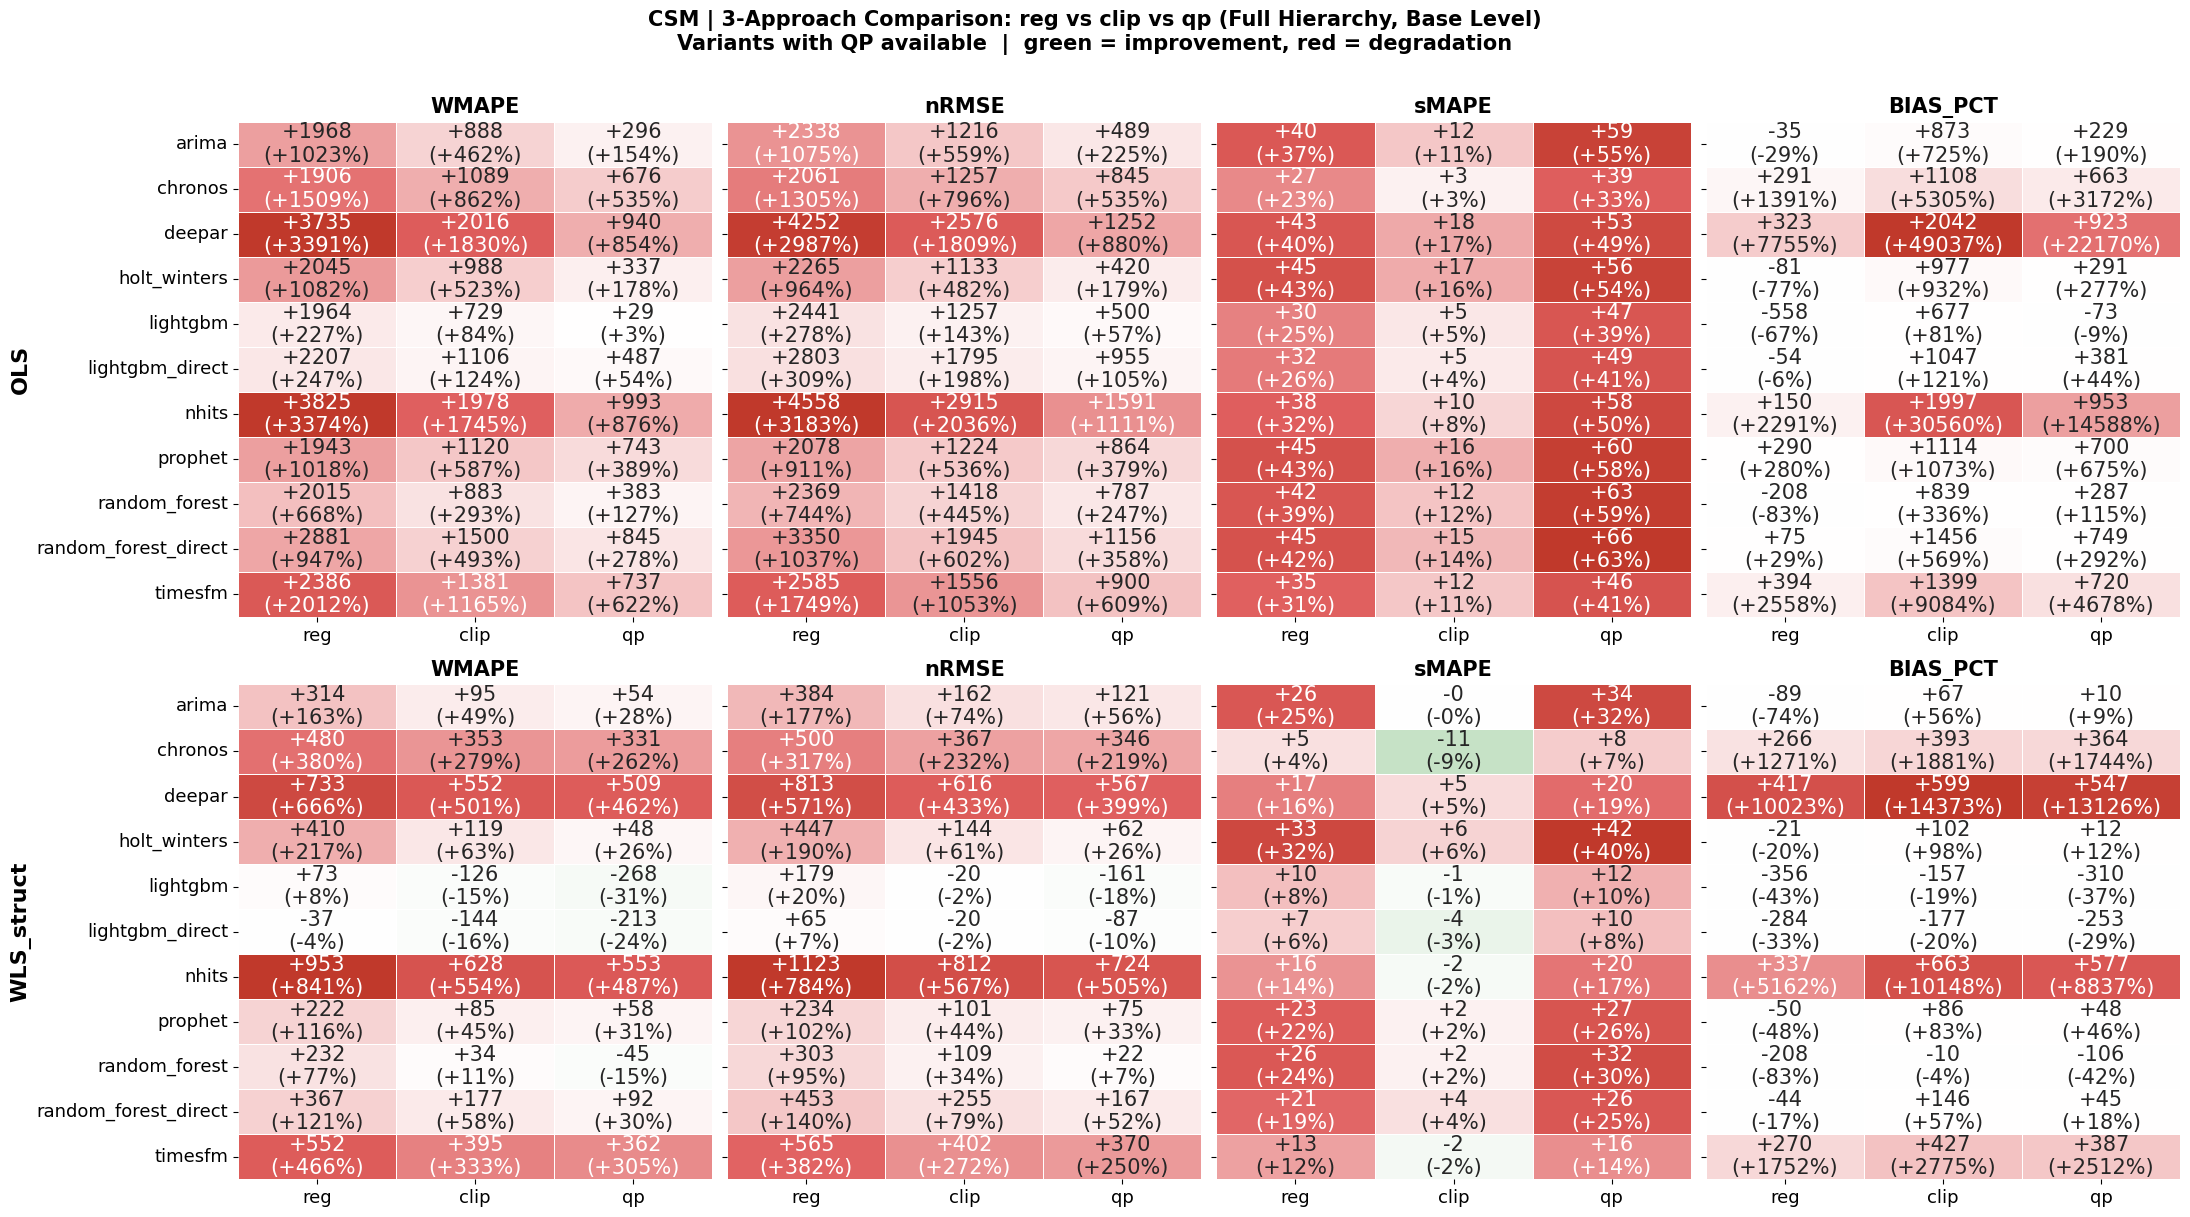
\includegraphics[width=1\textwidth]{slike/heatmap_csm_group1.png} 
    \caption{Структурно усклађивање (CSM): Промена перформанси након примене стабилних метода OLS и WLS\_Struct кроз три различита приступа.}
    \label{fig:csm_group1}
\end{figure}

\begin{figure}[htbp]
    \centering
     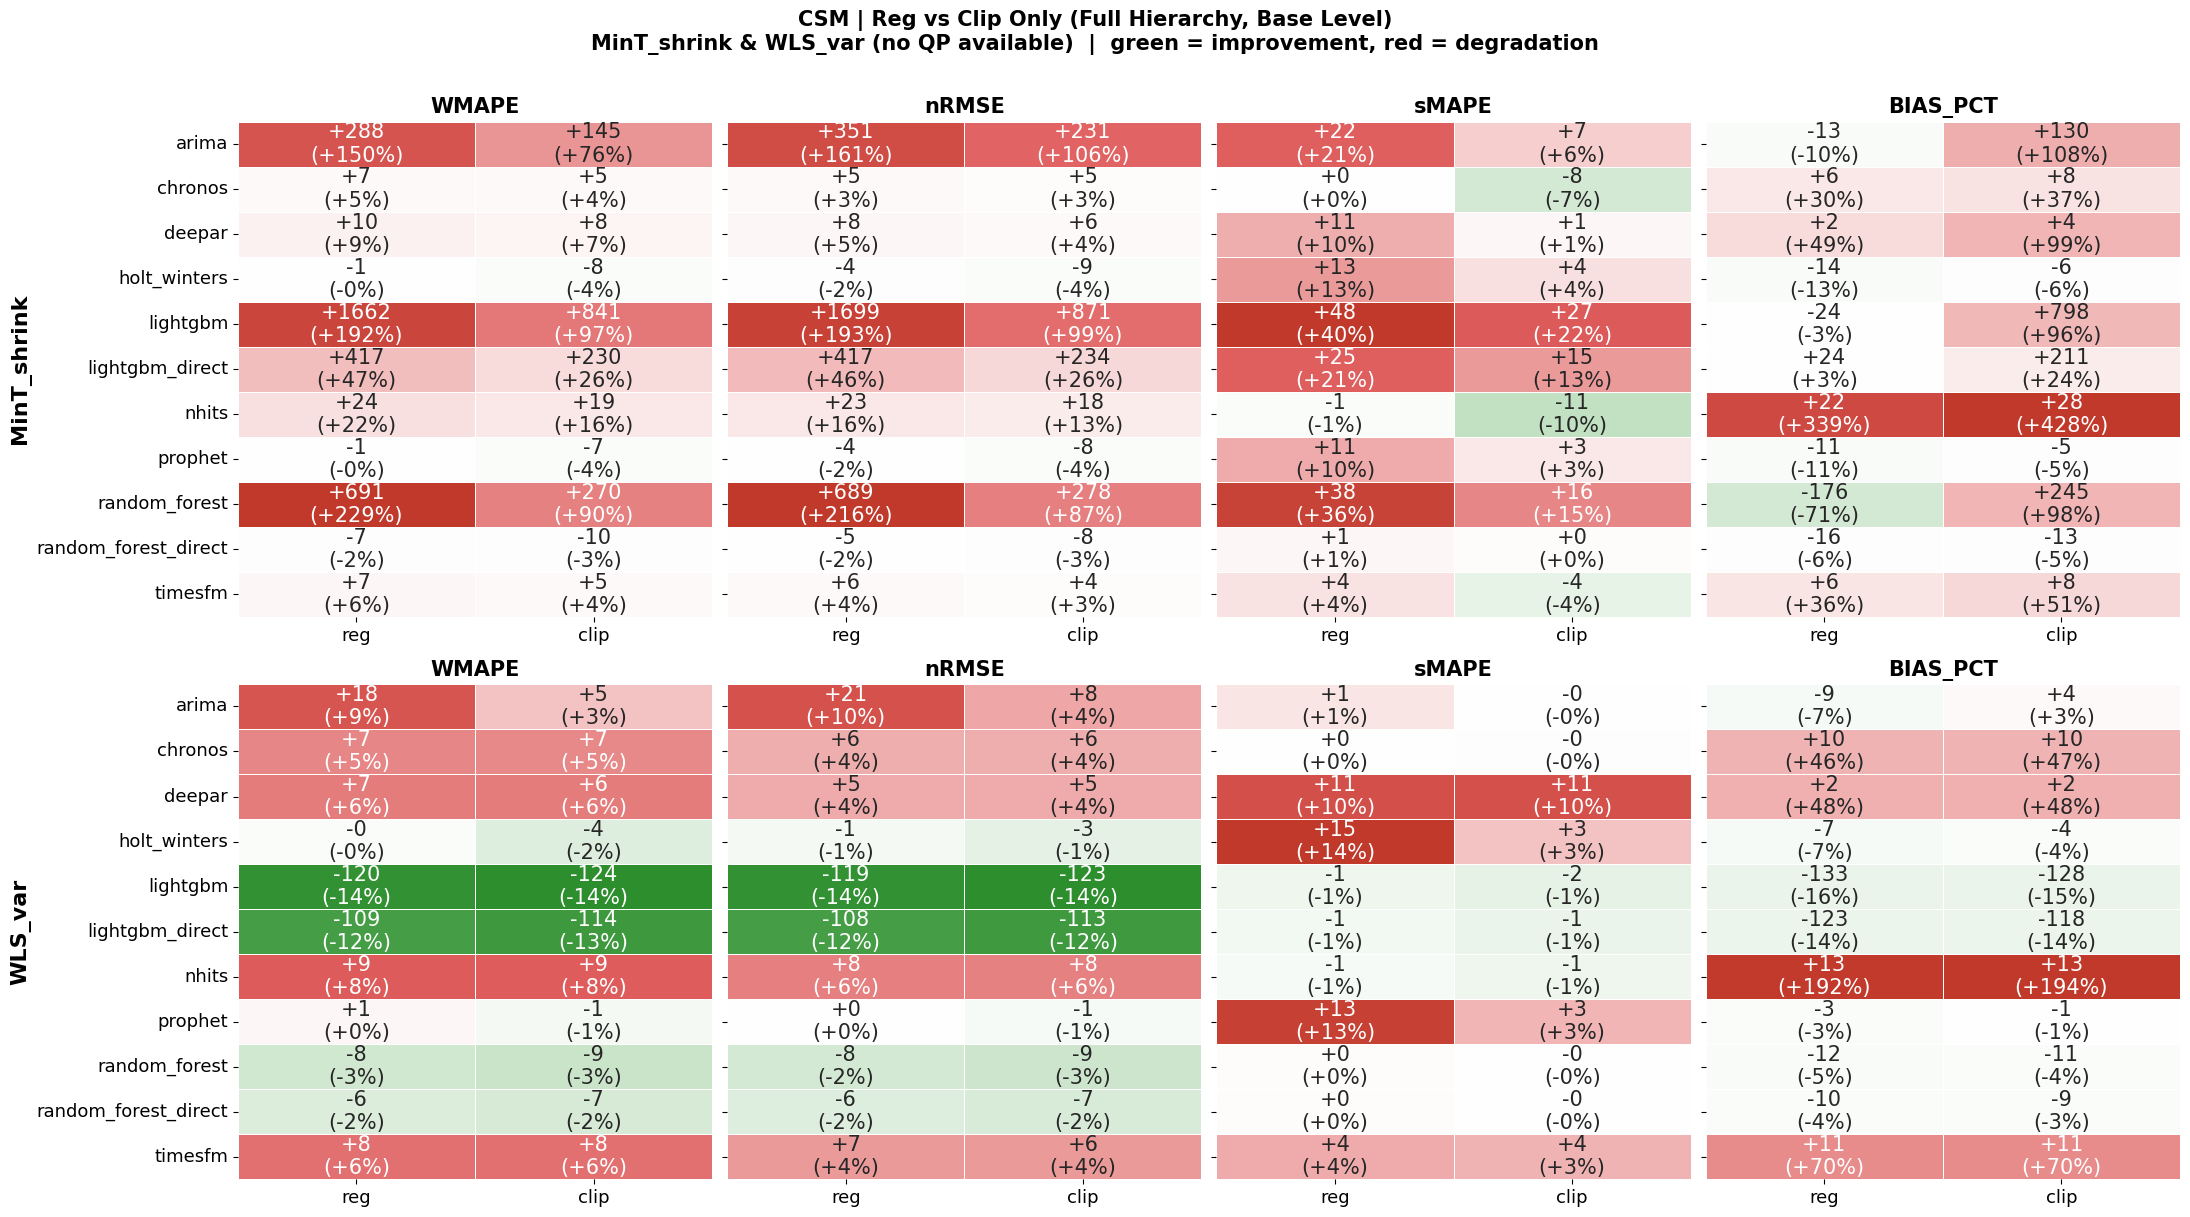
\includegraphics[width=1\textwidth]{slike/heatmap_csm_group2.png} 
    \caption{Структурно усклађивање (CSM): Промена перформанси након примене емпиријских метода MinT\_shrink и WLS\_var (QP оптимизација изостављена).}
    \label{fig:csm_group2}
\end{figure}

Анализа топлотних мапа за структурну димензију (слике \ref{fig:csm_group1} и \ref{fig:csm_group2}) открива један од најважнијих увида овог рада: \textbf{структурно усклађивање по правилу драстично деградира тачност прогноза на базном нивоу}.

Детерминистичка метода \textit{OLS} узрокује велику деградацију. На пример, код \textit{DeepAR} модела, OLS у неограниченом (\textit{reg}) режиму повећава $\mathrm{WMAPE}$ за екстремних $+3391\%$, док код \textit{Chronos} модела грешка расте за $+1509\%$. Овакав резултат је математички очекиван у системима са 20.000 серија: матрица \textit{OLS} претпоставља да све серије имају исту варијансу грешке, те слепо дистрибуира корекције са виших нивоа на ниже, потпуно уништавајући квалитетне локалне сигнале.

Примена методе \textit{WLS\_Struct} значајно ублажава ову деградацију (нпр. $\mathrm{WMAPE}$ за \textit{DeepAR} расте за $+666\%$), али и даље не доноси побољшање. Слично се понаша и \textit{MinT\_Shrink} метода, код које квалитетни базни модели попут \textit{Chronos}-а и \textit{DeepAR}-а бележе благи пад тачности (око $+5\%$ до $+9\%$).

Једини изузетак који показује висок ниво стабилности јесте метода \textbf{WLS\_Var}. Код ове методе, одлични модели задржавају своје перформансе уз минималну деградацију (нпр. \textit{Chronos} $\mathrm{WMAPE} +5\%$), док изразито лоши модели попут \textit{LightGBM}-а доживљавају оштро побољшање ($-14\%$). Овај налаз сугерише да је за успешно структурно усклађивање испрекиданих временских серија есенцијално скалирање корекција искључиво на основу историјске варијансе сваке појединачне серије, чиме се спречава преливање туђег шума на квалитетне прогнозе.

\begin{figure}[htbp]
    \centering
    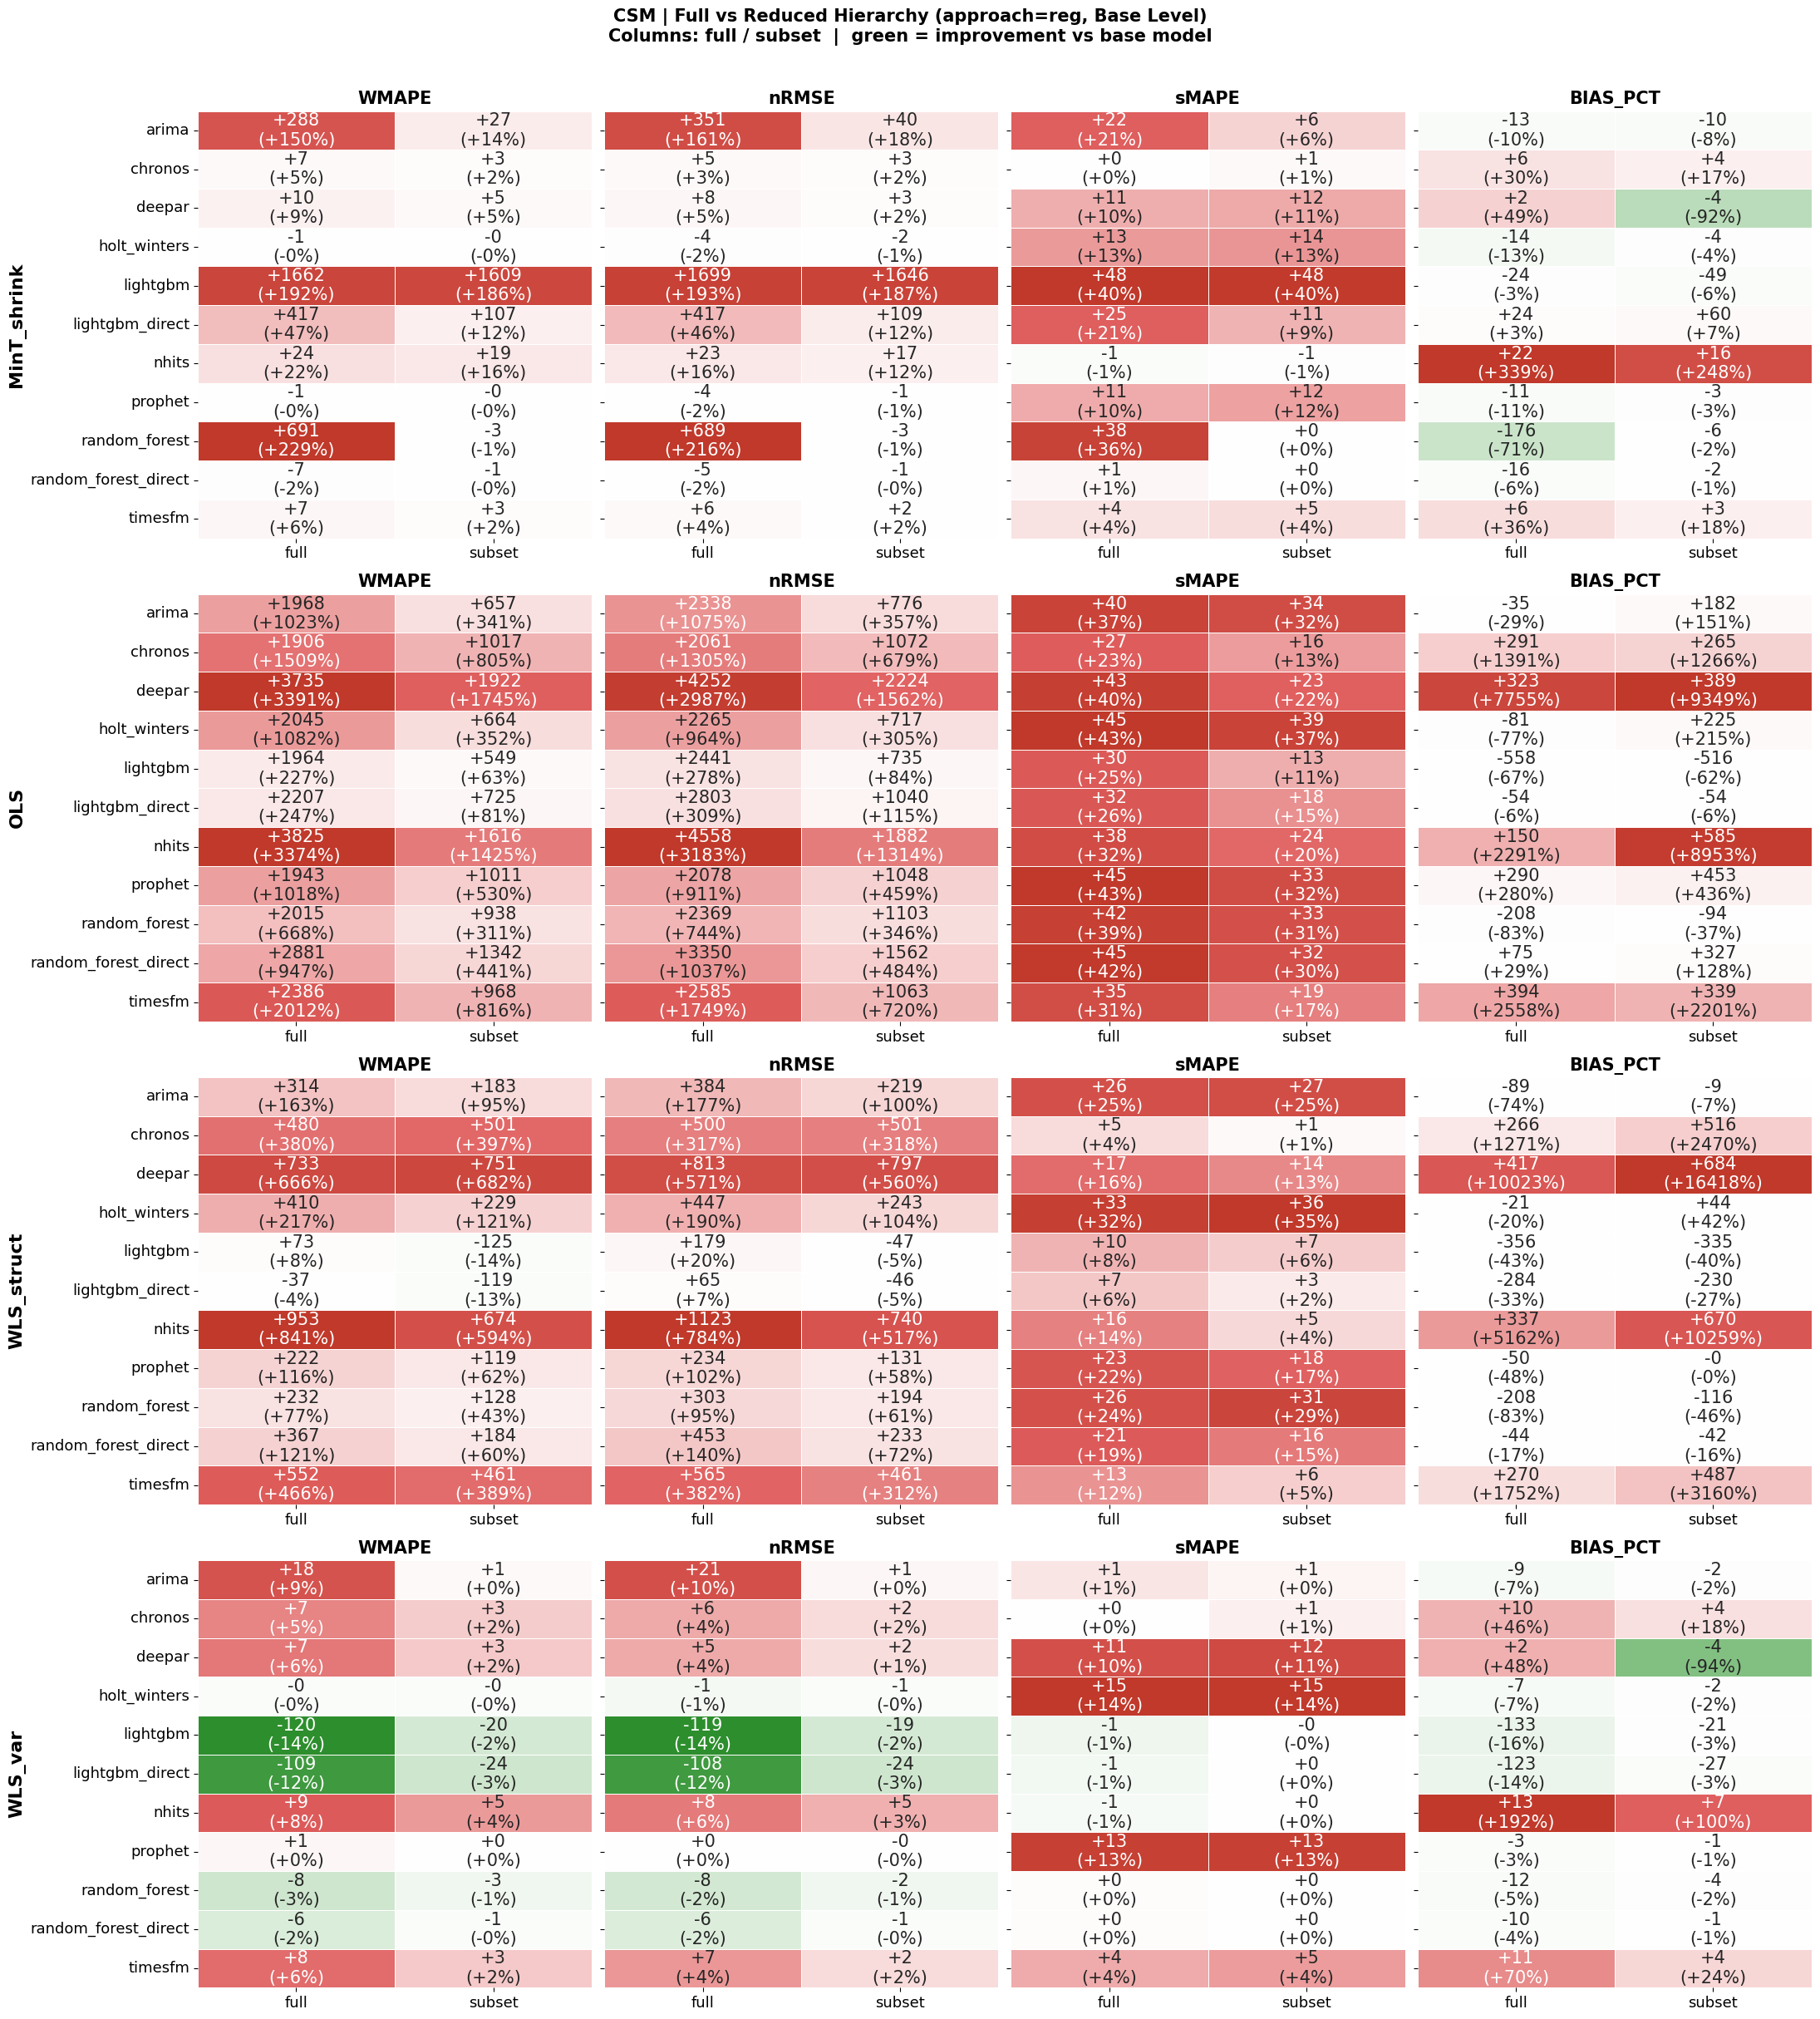
\includegraphics[width=1\textwidth]{slike/hierarchy_comparison.png} 
    \caption{Утицај дубине структурне хијерархије (Пуна наспрам Редуковане) на деградацију базних прогноза.}
    \label{fig:hierarchy_depth}
\end{figure}

\vspace{1em}
\noindent \textbf{Утицај дубине хијерархије:} \\
Додатни експеримент са редукованом структурном хијерархијом (Слика \ref{fig:hierarchy_depth}) показао је да уклањање нивоа \textit{купац}, \textit{производна хијерархија 2} и \textit{производна хијерархија 3} ублажава негативне ефекте усклађивања. На пример, деградација \textit{ARIMA} модела при \textit{OLS}-у пада са $+1023\%$ на $+341\%$. Мањи број нивоа значи мањи број степени слободе и мање веза у матрици сабирања $\mathbf{S}$, чиме се ограничава могућност алгоритма да прилагођава базне серије како би задовољио збирове на удаљеним нивоима.

\subsection{Временско усклађивање}

\begin{figure}[htbp]
    \centering
    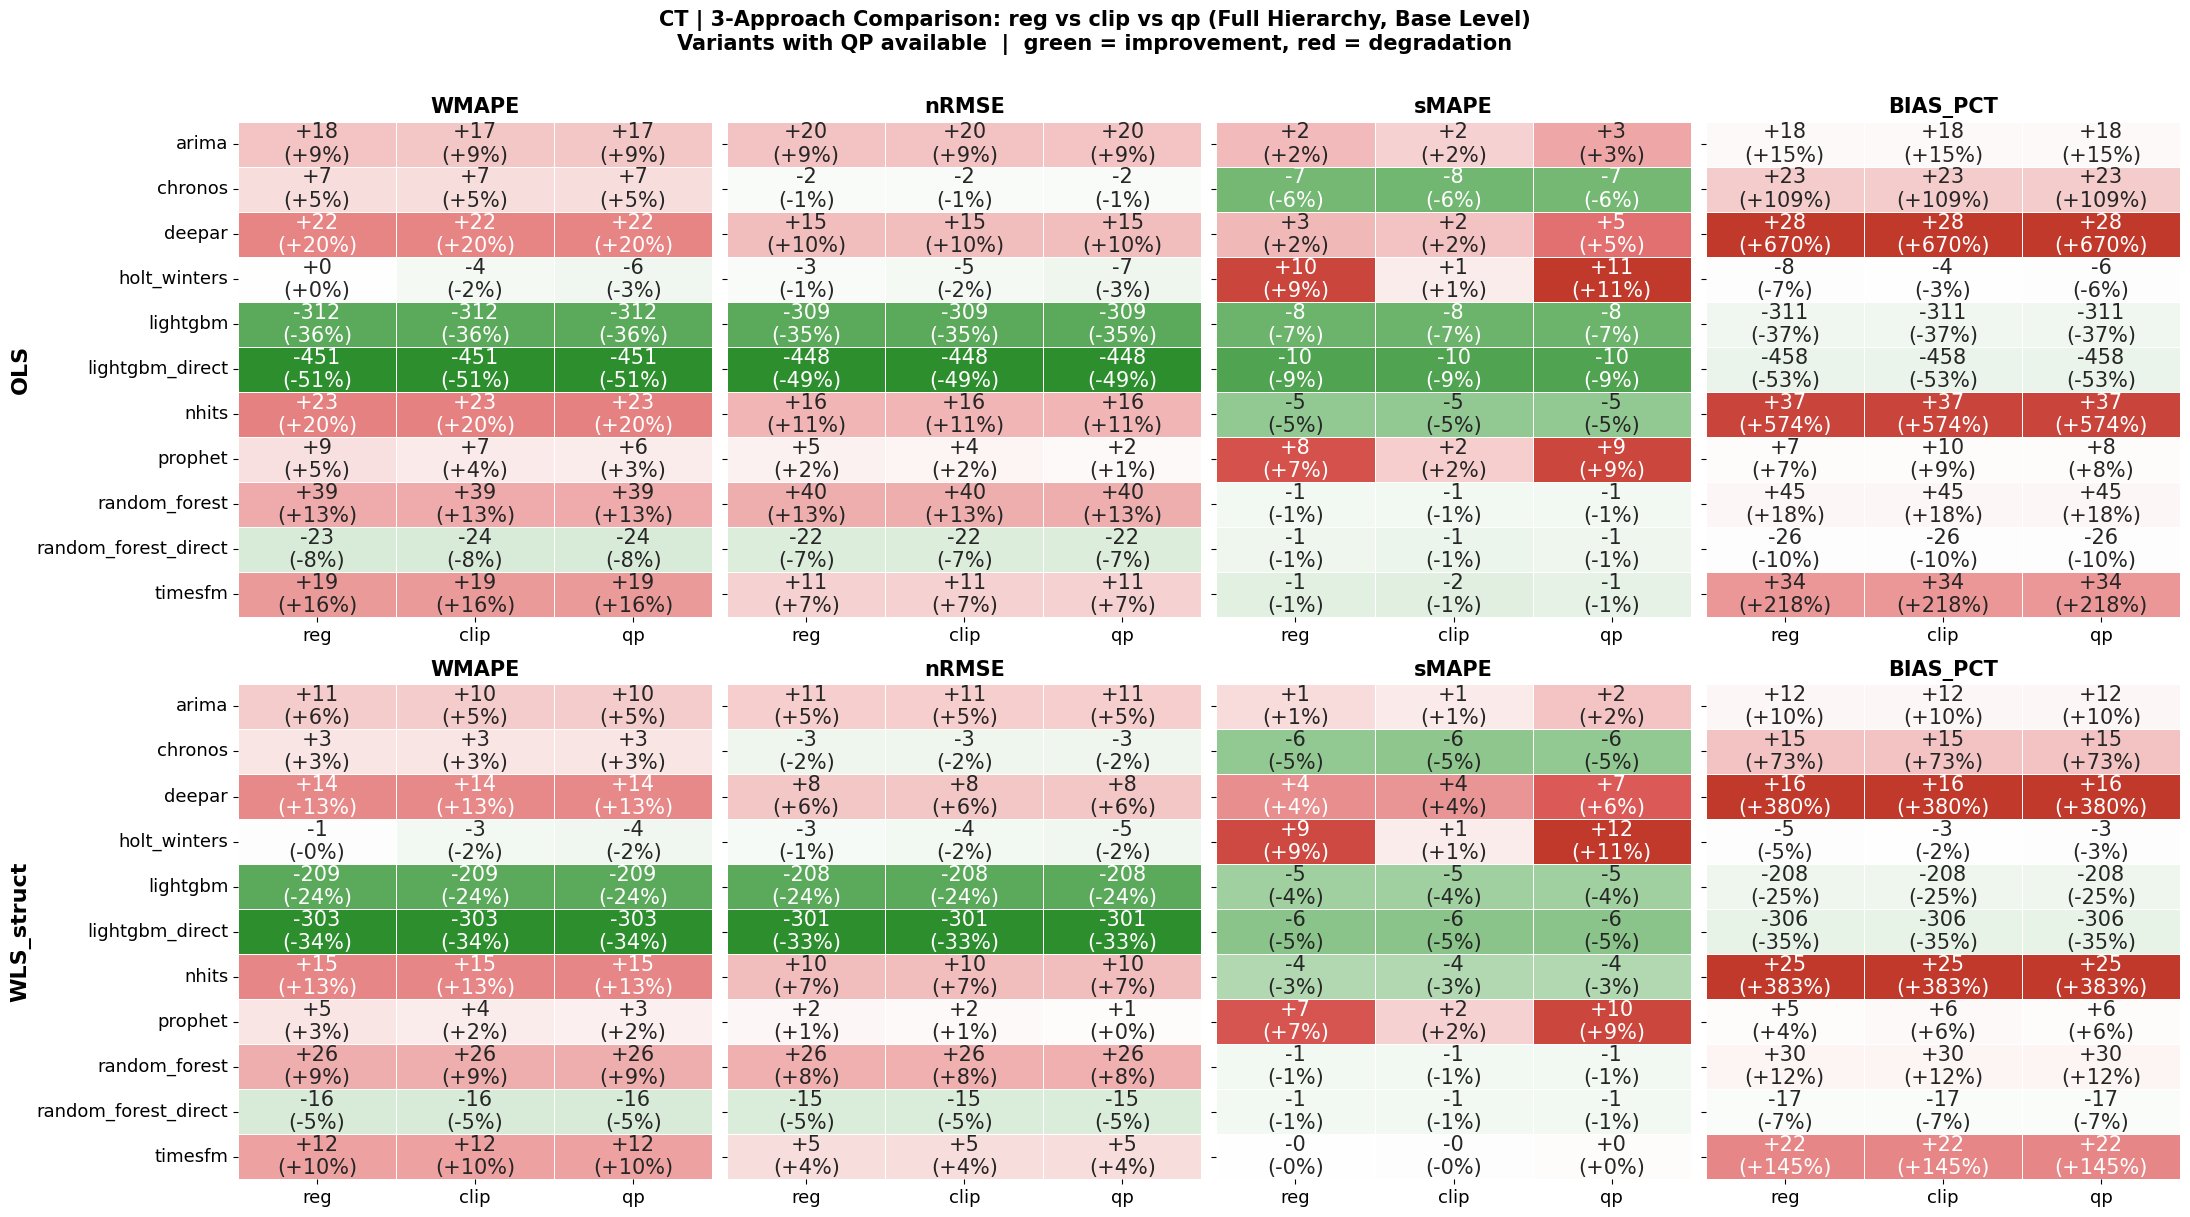
\includegraphics[width=1\textwidth]{slike/heatmap_ct_group1.png} 
    \caption{Временско усклађивање (CT): Промена перформанси након примене стабилних метода OLS и WLS\_Struct кроз три различита приступа.}
    \label{fig:ct_group1}
\end{figure}

\begin{figure}[htbp]
    \centering
    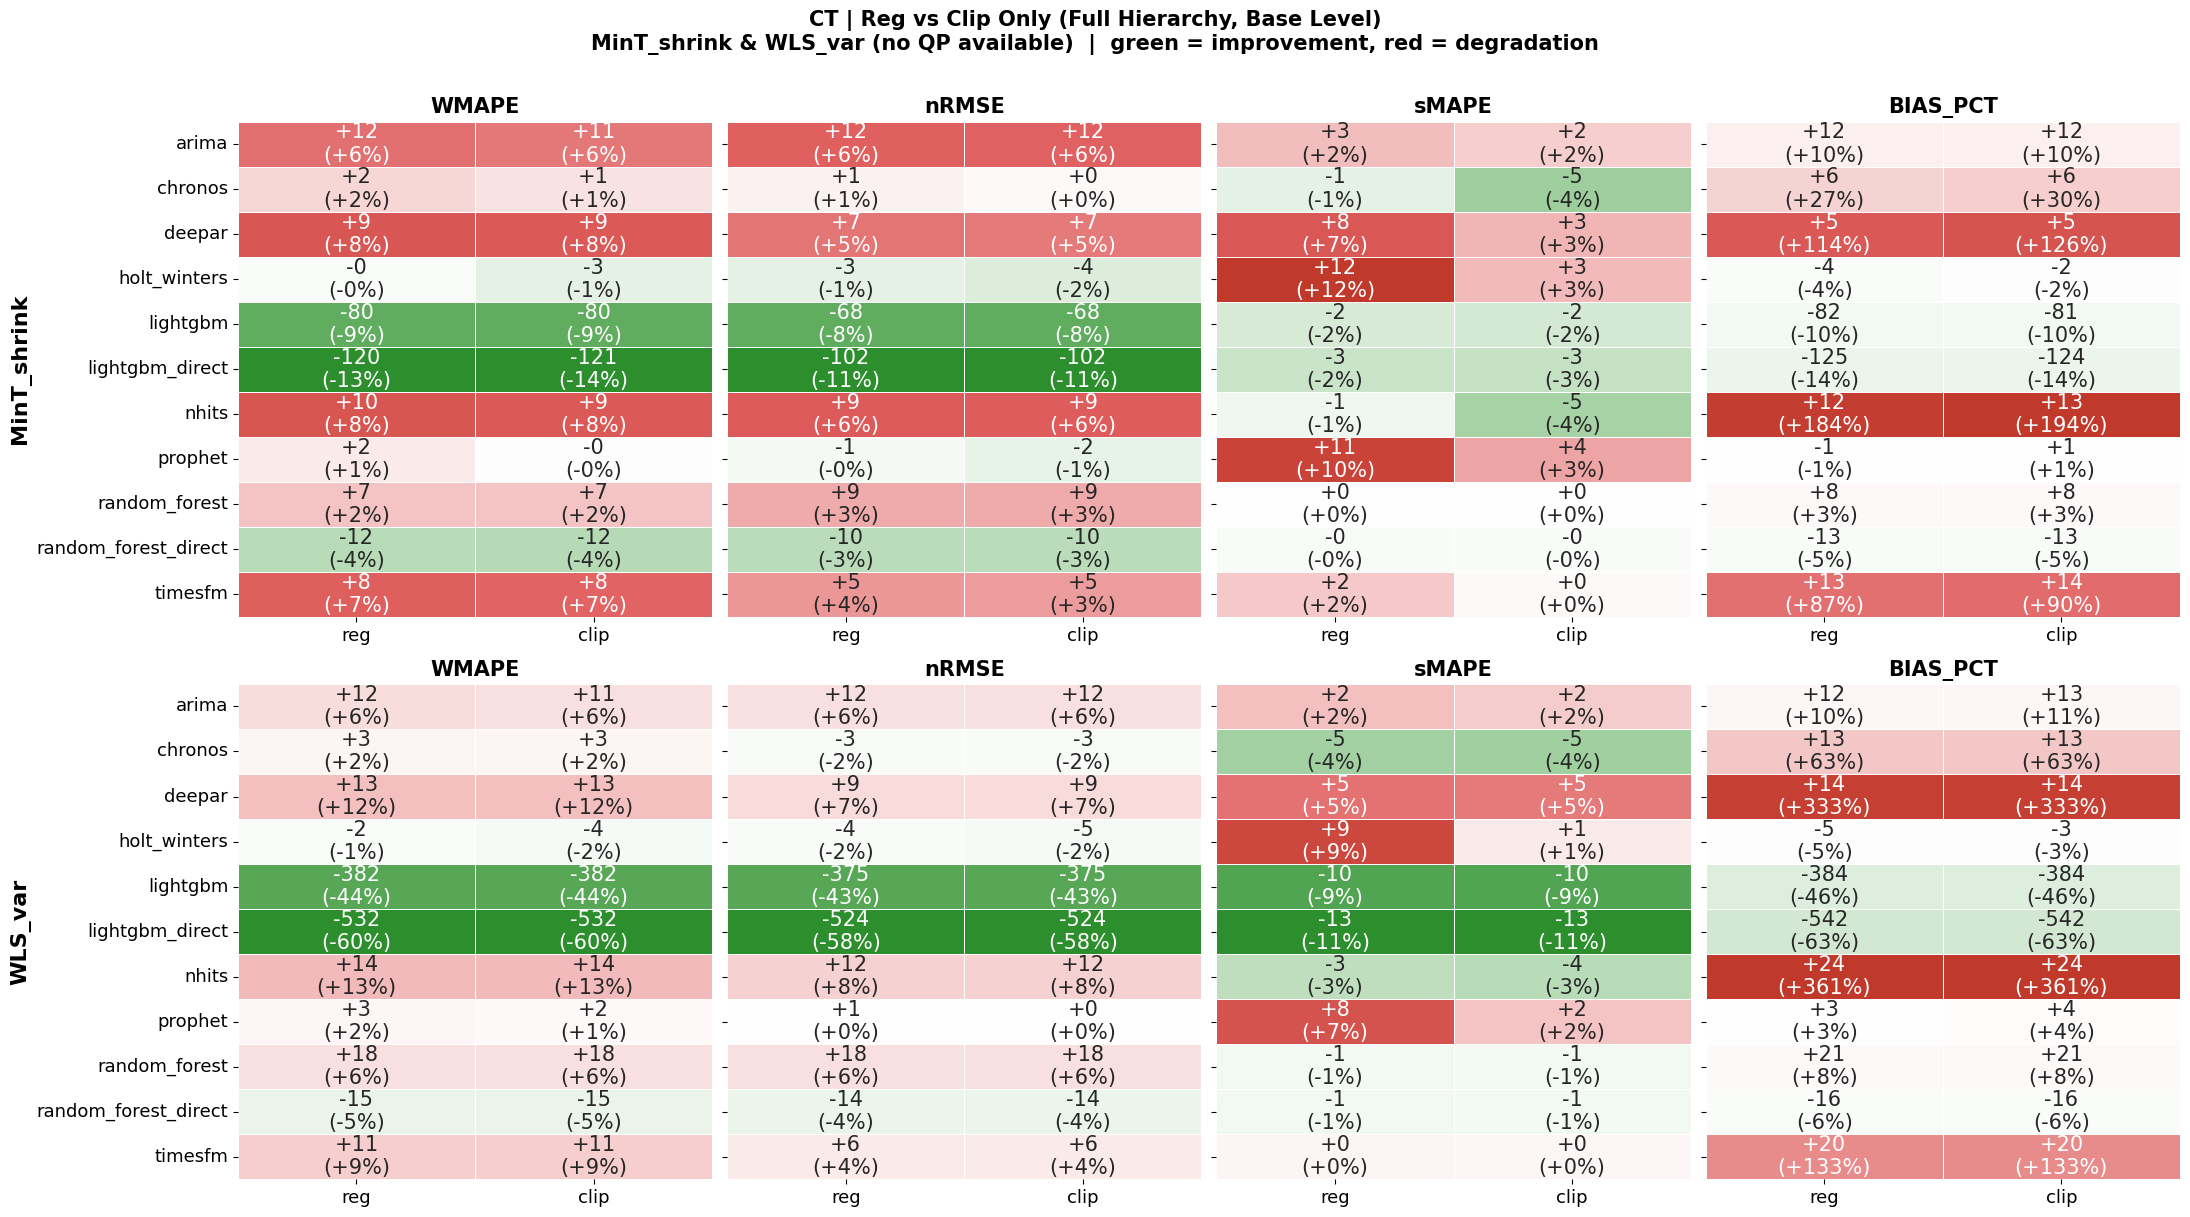
\includegraphics[width=1\textwidth]{slike/heatmap_ct_group2.png} 
    \caption{Временско усклађивање (CT): Промена перформанси након примене емпиријских метода MinT\_shrink и WLS\_var.}
    \label{fig:ct_group2}
\end{figure}

За разлику од структурног усклађивања, темпорална димензија (прелазак са месечне на кварталну агрегацију) манифестује потпуно другачије обрасце понашања.

Прво, резултати за сва три приступа (\textit{reg}, \textit{clip}, \textit{qp}) приказани на слици \ref{fig:ct_group1} су идентични код темпоралног усклађивања. Ово потврђује да агрегација из месечне у кварталну фреквенцију ретко или готово никада не генерише математички негативне прогнозе, те интервенције одсецања негативних вредности и квадратног програмирања нису имале никакав ефекат на систем.

Друго, темпорално усклађивање генерише снажна побољшања искључиво код најлошијих модела (нпр. \textit{LightGBM} бележи пад $\mathrm{WMAPE}$ метрике за $-36\%$ до $-60\%$). Овде је важно разумети саму механику алгоритма: MinT користи независно генерисане кварталне прогнозе како би кориговао месечне. Код лоших модела са високим нивоом шума, ове независне кварталне прогнозе су често релативно стабилније од месечних. Када алгоритам дистрибуира ту кварталну корекцију назад на месечни ниво, он ефективно врши пост-хок регуларизацију и смањује укупну грешку. Код детерминистичких метода (\textit{OLS}) ова дистрибуција је равномерна, док емпиријска метода \textit{WLS\_Var} ово ради интелигентно, тј. асиметрично коригује само оне месеце за које је модел историјски имао високу несигурност. Управо зато метода \textit{WLS\_Var} доноси и највеће побољшање за лоше моделе.

С друге стране, најбољи предиктивни модели (DeepAR, N-HITS, TimesFM) доживљавају деградацију (повећање $\mathrm{WMAPE}$ за $+10\%$ до $+20\%$) након темпоралног усклађивања. Ови модели већ генеришу оштре и прецизне локалне сигнале на месечном нивоу. Када алгоритам покуша да их усклади са њиховим кварталним прогнозама, он њихов квалитетан локални сигнал вештачки дистрибуира унутар квартала. Коначни закључак је да ефикасност темпоралног усклађивања директно зависи од количине шума у базним прогнозама: оно успешно регуларизује лоше калибрисане моделе, али истовремено доноси деградацију алгоритмима чији је базни сигнал већ оптималан. Стога се хијерархијско усклађивање у врхунским предиктивним системима не сме нужно посматрати као алат за смањење локалне грешке, већ примарно као административни механизам који обезбеђује пословну кохерентност целог система (која је неопходна за корпоративно извештавање и планирање буџета), при чему та кохерентност долази по цену благог пада прецизности на најнижем нивоу.


\section{Валидација и нарушавање хијерархијске кохерентности}

Као што је теоријски дефинисано у глави 2, основни циљ хијерархијског усклађивања је постизање агрегационе кохерентности система (збир прогноза деце мора бити једнак прогнози родитеља). Интерна евалуација на тест скупу потврдила је да неограничено усклађивање, као и усклађивање уз формална QP ограничења, остварују савршену структурну и темпоралну кохерентност ($100\%$ успешних провера над свим чворовима).

Међутим, примена хеуристичког одсецања негативних вредности подразумева нелинеарну трансформацију која неминовно нарушава ову математичку структуру. Како би се квантификовала цена овог инжењерског компромиса, спроведена је анализа. За сваки родитељски чвор упоређена је његова усклађена, а затим одсечена вредност са збиром усклађених, а затим одсечених вредности његових потомака са базног нивоа.

\begin{table}[htbp]
    \centering
    \caption{Просечно процентуално нарушавање кохерентности услед хеуристичког одсецања негативних вредности, приказано по нивоима агрегације.}
    \label{tab:coherence_loss}
    \vspace{0.5em}
    \begin{tabular}{l c c}
        \toprule
        \textbf{Ниво} & \textbf{Утицај (бр. чворова)} & \textbf{Нарушавање кохерентности (\%)} \\
        \midrule
        \textit{укупно} & 66.7\% & 6.92\% \\
        \textit{пословна област} & 47.6\% & 6.80\% \\
        \textit{локација} & 48.6\% & 6.55\% \\
        \textit{производна хијерархија 1} & 36.1\% & 6.04\% \\
        \textit{купац} & 38.1\% & 5.81\% \\
        \textit{производна хијерархија 2} & 27.3\% & 5.11\% \\
        \textit{производна хијерархија 3} & 23.7\% & 4.82\% \\
        \midrule
        \textbf{Агрегатно} & \textbf{-} & \textbf{6.00\%} \\
        \bottomrule
    \end{tabular}
\end{table}

Кључни налази ове анализе, сумирани у табели \ref{tab:coherence_loss}, указују на следеће:
\begin{itemize}
    \item \textbf{Укупно нарушавање система:} Агрегатна процентуална грешка кохерентности на нивоу целог система износи \textbf{6.00\%}. Ово значи да се, у просеку, извештаји на вишим агрегационим нивоима разликују за $6\%$ од физичког збира базних резервних делова услед одсецања негативних прогноза.
    
    \item \textbf{Дистрибуција по нивоима:} Губитак кохерентности је израженији на највишим нивоима агрегације (укупни \textit{укупно} ниво $6.92\%$, \textit{пословна област} $6.80\%$). Спуштањем кроз производну хијерархију ка грануларнијим нивоима, ово одступање природно опада (\textit{производна хијерархија 3} ниво бележи одступање од $4.82\%$). Овај феномен је логичан, јер виши нивои сабирају већи број базних серија, чиме се кумулативни ефекат одсечених нула додатно појачава.
\end{itemize}

Поред агрегационих нивоа, ниво нарушавања кохерентности представља директну последицу интеракције између квалитета базног модела и коришћене матрице усклађивања. Ова динамика приказана је у табели \ref{tab:coherence_models_methods}.

\begin{table}[htbp]
    \centering
    \caption{Процентуално нарушавање кохерентности услед хеуристичког одсецања негативних вредности, приказано по базним моделима и примењеним методама усклађивања.}
    \label{tab:coherence_models_methods}
    \vspace{0.5em}
    \begin{tabular}{l c c c c}
        \toprule
        \textbf{Модел} & \textbf{OLS} & \textbf{WLS\_Struct} & \textbf{MinT\_Shrink} & \textbf{WLS\_Var} \\
        \midrule
        \textit{DeepAR} & 15.24 & 1.11 & 0.05 & 0.001 \\
        \textit{N-HITS} & 17.72 & 2.07 & 0.28 & 0.01 \\
        \textit{TimesFM} & 7.78 & 0.74 & 0.06 & 0.004 \\
        \textit{Chronos} & 6.04 & 0.57 & 0.03 & 0.003 \\
        \textit{Holt-Winters} & 9.15 & 2.53 & 0.67 & 0.48 \\
        \textit{Prophet} & 8.23 & 1.29 & 0.48 & 0.29 \\
        \textit{ARIMA} & 12.73 & 2.13 & 15.71 & 0.50 \\
        \textit{Random Forest} & 12.58 & 2.53 & 48.32 & 0.06 \\
        \textit{Random Forest (dir.)} & 16.59 & 2.52 & 0.11 & 0.04 \\
        \textit{LightGBM} & 13.37 & 2.19 & \textbf{81.91} & 0.16 \\
        \textit{LightGBM (dir.)} & 13.91 & 1.77 & \textbf{54.38} & 0.26 \\
        \bottomrule
    \end{tabular}
\end{table}

\begin{itemize}
    \item \textbf{Детерминистички приступ (OLS):} Ова метода је изразито нестабилна на свим моделима. Она слепо дистрибуира корекције и генерише велике негативне вредности чијим се одсецањем кохерентност трајно нарушава (конзистентно између $6\%$ и $17\%$).

    \item \textbf{Структурно скалирање (WLS\_Struct):} Ова метода представља стабилну средину. Коришћењем саме хијерархијске структуре за апроксимацију несигурности, она значајно ублажава екстреме у односу на \textit{OLS}. Без обзира на квалитет базног модела, задржава губитак кохерентности у уским и пословно прихватљивим границама (између $0.5\%$ и $2.5\%$).
    
    \item \textbf{Емпиријски приступи (WLS\_Var и MinT\_Shrink):} Метода \textit{WLS\_Var} доказује своју супериорност јер интелигентно скалира корекције према стварној варијанси серија, чиме се потреба за одсецањем негативних вредности и губитак кохерентности своде на ниво занемарљиве грешке (често испод $0.01\%$). Са друге стране, метода \textit{MinT\_Shrink} показује екстремну осетљивост на одударајуће податке: код квалитетних модела не квари збирове, али у комбинацији са изразито пристрасним \textit{LightGBM}-ом доводи до драматичног пада кохерентности (преко $80\%$ грешке).
\end{itemize}

\section{Дискусија добијених резултата}

Темељна евалуација на подацима из домена резервних делова преиспитује традиционалне претпоставке о хијерархијском усклађивању. Експеримент недвосмислено показује да усклађивање није универзално решење за побољшање предиктивне тачности. На подацима са великим уделом испрекиданих серија, агрегација уноси значајан ниво шума. Уколико се тај шум слепо дистрибуира назад на базни ниво (као код методе \textit{OLS}), долази до велике деградације локалних сигнала. Када систем користи врхунске алгоритме дубоког учења или вишенаменске претрениране моделе, њихове базне прогнозе су већ толико добро калибрисане да им линеарно усклађивање са вишим нивоима готово уопште не помаже, већ их благо погоршава.

Значајан аспект дискусије односи се на утицај дубине, односно дизајна саме структурне хијерархије и на квалитет усклађених прогноза. Поређење пуне и редуковане хијерархије недвосмислено показује да комплекснија структура, са већим бројем међунивоа (агрегационих погледа), уноси додатну грешку у систем. Сваки нови ниво уводи додатна ограничења која базне серије морају да задовоље, што алгоритам приморава на непотребну адаптацију локалних сигнала како би се поклопили са удаљеним збировима. Смањењем броја агрегационих погледа (редукована хијерархија), ефективно се смањује број степени слободе у пројекционој матрици, чиме се значајно ублажава деградација базних прогноза. Ово потврђује да дизајн хијерархије не сме бити вођен искључиво организационим корпоративним шемама, већ се мора пажљиво балансирати како алгебарска ограничења не би преоптеретила предиктивни систем.

Ефекат темпоралног усклађивања захтева посебно опрезну интерпретацију. Уместо простог математичког усредњавања,  алгоритам темпоралног усклађивања користи независно генерисане агрегиране (кварталне) прогнозе како би кориговао базне (месечне) сигнале. Детаљна анализа открива да овај процес суштински функционише као механизам пост-хок регуларизације. Дистрибуцијом кварталних вредности наниже, алгоритам ефективно ублажава екстремне локалне осцилације и велику пристрасност лоших модела, чиме им стварно и значајно смањује укупну грешку. Међутим, инхерентна цена ове регуларизације је вештачко погоршавање већ прецизних локалних сигнала код висококвалитетних модела. Због тога, закључак да темпорално усклађивање побољшава систем у просеку заправо представља последицу екстремних поправки најлошијих модела. У реалности, напредним алгоритмима ова врста темпоралне интервенције не доноси корист, већ доводи до благог пада њихове иницијалне прецизности.

Коначно, анализа доменских ограничења потврђује да је у индустријској пракси инжењерски компромис често бољи од строге математике. Иако формално квадратно програмирање (QP) гарантује кохерентност без одсецања негативних вредности, његова рачунарска нестабилност чини га неупотребљивим за системе са 20.000 серија. Хеуристичко одсецање негативних вредности на нулу успешно решава овај проблем уз занемарљиву цену: упарен са интелигентном методом \textit{WLS\_Var}, он нарушава математичку кохерентност система за мање од $0.5\%$, што је у пословном извештавању углавном потпуно прихватљива маргина грешке.

\section{Идентификација најбољих пракси за дати проблем}

На основу синтезе резултата, дефинисане су конкретне инжењерске препоруке за пројектовање предиктивних система у описаном домену:

\begin{enumerate}
    \item \textbf{Избор алгоритама:} Приоритет треба дати моделима дубоког учења (\textit{DeepAR}) или вишенаменским претренираним моделима (\textit{Chronos}, \textit{TimesFM}) посебно ако нам је потребно да брзо дођемо до иницијалних резултата. Класична стабла одлучивања (\textit{LightGBM}, \textit{Random Forest}) не треба користити на скупу са великим уделом испрекиданих временских серија без претходне промене функције циља и конструкције карактеристика.
    
    \item \textbf{Стратегија примене усклађивања:} Одлука о димензији усклађивања мора бити директно вођена пословним приоритетима:
    \begin{itemize}
        \item Уколико је \textbf{максимална тачност на базном нивоу} апсолутни приоритет (нпр. за аутоматизовано наручивање делова), а користе се квалитетни модели, хијерархијско усклађивање треба \textbf{потпуно избегавати}.
        \item Уколико су \textbf{кохерентни извештаји} неопходни за менаџмент, применити структурно усклађивање, али искључиво кроз методу \textbf{\textit{WLS\_Var}}, и уз пажљив избор хијерархија, како би се сачувао интегритет добрих базних модела.
        \item Темпорално усклађивање треба стратешки користити искључиво као механизам пост-хок регуларизације у системима где се нужно користе лошији, нестабилни модели са високом варијансом. За добре моделе, темпорално усклађивање не доноси побољшања.
    \end{itemize}
    
    \item \textbf{Третман негативних прогноза:} Уместо нумерички нестабилних QP решавача, препоручује се неограничено усклађивање праћено хеуристичким одсецањем негативних вредности на нулу. Упарен са методом WLS\_Var, овај приступ нуди максималну стабилност уз занемарљив губитак кохерентности.
    
    \item \textbf{Дизајн хијерархије:} Комплексност агрегације треба свести на апсолутни минимум. Увођење непотребних међунивоа у структурну хијерархију повећава број степени слободе и доводи до прекомерних, штетних корекција базних серија.
\end{enumerate}

% ------------------------------------------------------------------------------
\chapter{Закључак}
\label{chp:zakljucak}
% ------------------------------------------------------------------------------

\section{Синтеза кључних налаза истраживања}

У овом мастер раду спроведена је свеобухватна анализа утицаја хијерархијског усклађивања на прецизност предвиђања временских серија, мотивисана индустријским проблемом предвиђања потражње резервних делова. Специфичност овог домена огледа се у високој димензионалности, сложеној структури агрегације и великом уделу испрекиданих временских серија.

Најзначајнији допринос овог рада лежи у побијању претпоставке да хијерархијско усклађивање аутоматски побољшава локалну прецизност модела. Резултати недвосмислено доказују да врхунски алгоритми, посебно вишенаменски претренирани модели (\textit{Chronos}, \textit{TimesFM}) и вероватносне неуронске мреже (\textit{DeepAR}), екстрахују максимум релевантних информација директно из сирових података. Накнадно линеарно усклађивање таквих добро калибрисаних локалних сигнала са независним агрегираним нивоима кроз алгоритме MinT не доноси корист, већ често уноси грешку. За високо прецизне моделе, хијерархијско усклађивање се стога мора посматрати превасходно као неопходан административни механизам за корпоративно извештавање, а не као алатка за минимизацију локалне грешке.

Значајан налаз ове студије је и директан утицај самог дизајна хијерархије на резултате усклађивања. Показано је да комплекснија структура са већим бројем агрегационих погледа уноси додатну грешку у систем. Редукована хијерархија (са мањим бројем нивоа) показала се као боља, јер смањење броја степени слободе у матрици сабирања ефективно ограничава нежељено прилагођавање базних серија.

Поред тога, рад се дотакао и решавања конфликта између строге математичке кохерентности и пословних ограничења (ненегативности). Показали смо да је у високодимензионалним системима замена нестабилне формалне оптимизације (QP) рачунарски јефтиним хеуристикама (одсецање негативних вредности на нулу) неопходна за физичку употребљивост прогноза. Упарен са методама које поштују историјску варијансу (попут \textit{WLS\_Var}), овај инжењерски компромис чува агрегациони интегритет система уз занемарљив губитак математичке кохерентности.


\section{Ограничења спроведене анализе}

Као и свако истраживање, и ово има своја ограничења која треба узети у обзир приликом интерпретације резултата.

Прво ограничење односи се на рачунарске и математичке ресурсе при раду са високодимензионалним системима. Због екстремне меморијске захтевности, није било могуће извршити експлицитну алокацију велике матрице за истовремено (заједничко) структурно и темпорално усклађивање над 20.000 серија. Такође, због природе података где је број серија знатно већи од броја доступних временских корака ($n \gg T$), математички је немогуће инвертовати пуну емпиријску матрицу коваријансе. Због тога није било могуће тестирати класични алгоритам MinT.

Друго ограничење везано је за моделе класичног машинског учења (\textit{LightGBM}, \textit{Random Forest}). Ови алгоритми су намерно тренирани искључиво са историјским и календарским карактеристикама, уз стандардну MSE функцију циља. Разлог за овако скроман избор улазних података било је фер поређење са статистичким и вишенаменским претренираним моделима, којима је доступна искључиво историја циљне променљиве. Иако је тиме спречено да се моделима заснованим на стаблима даје предност кроз екстерне информације, то уједно значи да приказане перформансе ових алгоритама у раду не представљају њихов теоријски максимум.

Коначно, важно је нагласити да су сви закључци изведени на специфичном скупу података из домена потражње резервних делова, који одликује екстремна испрекиданост и велики број нултих вредности. Ови резултати се не могу аутоматски генерализовати; постоји велика вероватноћа да би на "глатким" временским серијама са стабилним и великим волуменом продаје (нпр. у класичној малопродаји робе широке потрошње) линеарно усклађивање кроз алгоритме MinT дало значајно другачије, вероватно повољније резултате.


\section{Препоруке за будућа истраживања и практичну примену}

Претходно наведена ограничења директно инспиришу и дефинишу правце за будућа истраживања. Када је реч о предиктивном моделовању, логичан наредни корак био би развој модела заснованих на стаблима кроз имплементацију прилагођених функција губитка  и увођење богатијег скупа екстерних карактеристика. Ово би омогућило да се испита да ли ти алгоритми могу да парирају вишенаменским претренираним моделима када нису ограничени. Такође, репликација ове експерименталне поставке на скуповима "глатких" временских серија високог волумена омогућила би компаративну анализу понашања алгоритама MinT у суштински различитим тржишним условима.

У домену алгоритмике усклађивања, будућа истраживања би се могла фокусирати на технике смањења димензионалности које би омогућиле апроксимацију класичног MinT приступа чак и када је $N \gg T$, као и на алгоритамску оптимизацију меморијских захтева за заједничко структурно-временско усклађивање. Код вероватносних модела фокус би се могао померити на вероватносно усклађивање, где би се кроз хијерархију уместо тачкастих прогноза пројектовале целе вероватносне расподеле. Такође, постоји огроман потенцијал у интеграцији најновијих парадигми неуронског усклађивања (енг. \textit{neural reconciliation}) \cite{mancuso2021machine}. Уместо ослањања на фиксне линеарне пројекције (попут матрица MinT), ови савремени приступи користе архитектуре попут аутоенкодера или потпуно повезаних мрежа како би директно из података научили оптималне, нелинеарне пресликавајуће функције. Имплементација оваквих нелинеарних алгоритама представља један од најперспективнијих праваца тренутно.

Резултати истраживања дају увид у то како избор методе усклађивања утиче на тачност предвиђања, математичку кохерентност и рачунарску стабилност, што може бити корисно за пројектовање робусних предиктивних система.


% ------------------------------------------------------------------------------
% Literatura
% ------------------------------------------------------------------------------
\literatura

% ==============================================================================
% Završni deo teze i prilozi
\backmatter
% ==============================================================================

% ------------------------------------------------------------------------------
% Biografija kandidata
% \begin{biografija}
% \end{biografija}
% ------------------------------------------------------------------------------

\end{document} 